% uWaterloo Thesis Template for LaTeX 
% Last Updated May 24, 2011 by Stephen Carr, IST Client Services
% FOR ASSISTANCE, please send mail to rt-IST-CSmathsci@ist.uwaterloo.ca

% --------------------- Start of Document Preamble -----------------------

% Specify the document class, default style attributes, and page dimensions
% For hyperlinked PDF, suitable for viewing on a computer, use this:
\documentclass[letterpaper,12pt,titlepage,oneside,final]{book} % default value for 'report' class is "2"

% For PDF, suitable for double-sided printing, change the PrintVersion variable below
% to "true" and use this \documentclass line instead of the one above:
%\documentclass[letterpaper,12pt,titlepage,openright,twoside,final]{book}

% Some LaTeX commands I define for my own nomenclature.
% If you have to, it's better to change nomenclature once here than in a 
% million places throughout your thesis!
\newcommand{\package}[1]{\textbf{#1}} % package names in bold text
\newcommand{\cmmd}[1]{\textbackslash\texttt{#1}} % command name in tt font 
\newcommand{\href}[1]{#1} % does nothing, but defines the command so the
% print-optimized version will ignore \href tags (redefined by hyperref pkg).
%\newcommand{\texorpdfstring}[2]{#1} % does nothing, but defines the command
% Anything defined here may be redefined by packages added below...

% This package allows if-then-else control structures.
\usepackage{ifthen}
\newboolean{PrintVersion}
\setboolean{PrintVersion}{false} 
% CHANGE THIS VALUE TO "true" as necessary, to improve printed results for hard copies
% by overriding some options of the hyperref package below.

%\usepackage{nomencl} % For a nomenclature (optional; available from ctan.org)
\usepackage{amsmath,amssymb,amstext} % Lots of math symbols and environments
\usepackage[pdftex]{graphicx} % For including graphics N.B. pdftex graphics driver 
%\usepackage[Sonny]{fncychap}

\usepackage[hang]{footmisc}
% Hyperlinks make it very easy to navigate an electronic document.
% In addition, this is where you should specify the thesis title
% and author as they appear in the properties of the PDF document.
% Use the "hyperref" package 

\usepackage{lipsum}
\usepackage{listings}
\usepackage{placeins}
\usepackage{algorithm}
\usepackage{algpseudocode}

\usepackage{tablefootnote}
\usepackage{enumitem}
\usepackage{dirtree}
\usepackage{boldline}
\usepackage{pdfpages}
\usepackage{multirow}
\usepackage{tabularx, booktabs}
\usepackage{subcaption}
\usepackage{hhline}
\usepackage{array}
\usepackage{tabularx}
\usepackage{longtable}
\usepackage{ltxtable}

\newenvironment{blockquote}{%
	\par%
	\medskip
	\leftskip=4em\rightskip=2em%
	\noindent\ignorespaces}{%
	\par\medskip}



% N.B. HYPERREF MUST BE THE LAST PACKAGE LOADED; ADD ADDITIONAL PKGS ABOVE
\usepackage[pdftex,pagebackref=false]{hyperref} % with basic options
%\usepackage{hyperref}
% N.B. pagebackref=true provides links back from the References to the body text. This can cause trouble for printing.
\hypersetup{
	plainpages=false,       % needed if Roman numbers in frontpages
	unicode=false,          % non-Latin characters in Acrobat’s bookmarks
	pdftoolbar=true,        % show Acrobat’s toolbar?
	pdfmenubar=true,        % show Acrobat’s menu?
	pdffitwindow=false,     % window fit to page when opened
	pdfstartview={FitH},    % fits the width of the page to the window
	pdftitle={Curisoisty-Based Reinforcement Learning Algorithm for Interactive Art Sculptures},    % title: CHANGE THIS TEXT!
	    pdfauthor={Matthew Tsz Kiu Chan},  
%	    pdfsubject={Subject},  % subject: CHANGE THIS TEXT! and uncomment this line
%	    pdfkeywords={keyword1} {key2} {key3}, % list of keywords, and uncomment this line if desired
	pdfnewwindow=true,      % links in new window
	colorlinks=true,        % false: boxed links; true: colored links
	linkcolor=blue,         % color of internal links
	citecolor=green,        % color of links to bibliography
	filecolor=magenta,      % color of file links
	urlcolor=cyan           % color of external links
}
\ifthenelse{\boolean{PrintVersion}}{   % for improved print quality, change some hyperref options
	\hypersetup{	% override some previously defined hyperref options
		%    colorlinks,%
		citecolor=black,%
		filecolor=black,%
		linkcolor=black,%
		urlcolor=black}
}{} % end of ifthenelse (no else)

% Setting up the page margins...
% uWaterloo thesis requirements specify a minimum of 1 inch (72pt) margin at the
% top, bottom, and outside page edges and a 1.125 in. (81pt) gutter
% margin (on binding side). While this is not an issue for electronic
% viewing, a PDF may be printed, and so we have the same page layout for
% both printed and electronic versions, we leave the gutter margin in.
% Set margins to minimum permitted by uWaterloo thesis regulations:
\setlength{\marginparwidth}{0pt} % width of margin notes
% N.B. If margin notes are used, you must adjust \textwidth, \marginparwidth
% and \marginparsep so that the space left between the margin notes and page
% edge is less than 15 mm (0.6 in.)
\setlength{\marginparsep}{0pt} % width of space between body text and margin notes
\setlength{\evensidemargin}{0.125in} % Adds 1/8 in. to binding side of all 
% even-numbered pages when the "twoside" printing option is selected
\setlength{\oddsidemargin}{0.125in} % Adds 1/8 in. to the left of all pages
% when "oneside" printing is selected, and to the left of all odd-numbered
% pages when "twoside" printing is selected
\setlength{\textwidth}{6.375in} % assuming US letter paper (8.5 in. x 11 in.) and 
% side margins as above
\raggedbottom


% The following statement specifies the amount of space between
% paragraphs. Other reasonable specifications are \bigskipamount and \smallskipamount.
\setlength{\parskip}{\medskipamount}

% The following statement controls the line spacing.  The default
% spacing corresponds to good typographic conventions and only slight
% changes (e.g., perhaps "1.2"), if any, should be made.
\renewcommand{\baselinestretch}{1} % this is the default line space setting

% By default, each chapter will start on a recto (right-hand side)
% page.  We also force each section of the front pages to start on 
% a recto page by inserting \cleardoublepage commands.
% In many cases, this will require that the verso page be
% blank and, while it should be counted, a page number should not be
% printed.  The following statements ensure a page number is not
% printed on an otherwise blank verso page.
\let\origdoublepage\cleardoublepage
\newcommand{\clearemptydoublepage}{%
	\clearpage{\pagestyle{empty}\origdoublepage}}
\let\cleardoublepage\clearemptydoublepage


\usepackage{cleveref}
\setlength{\footnotemargin}{10pt}



%======================================================================
%   L O G I C A L    D O C U M E N T -- the content of your thesis
%======================================================================
\begin{document}
	
	%----------------------------------------------------------------------
	% FRONT MATERIAL
	%----------------------------------------------------------------------
	% T I T L E   P A G E
% -------------------
% Last updated May 24, 2011, by Stephen Carr, IST-Client Services
% The title page is counted as page `i' but we need to suppress the
% page number.  We also don't want any headers or footers.
\pagestyle{empty}
\pagenumbering{roman}

% The contents of the title page are specified in the "titlepage"
% environment.
\begin{titlepage}
        \begin{center}
        \vspace*{1.0cm}

        \Huge
        {\bf Curiosity-Based Learning Algorithm for Interactive Art Sculptures}

        \vspace*{1.0cm}

        \normalsize
        by \\

        \vspace*{1.0cm}

        \Large
        Matthew Tsz Kiu Chan \\

        \vspace*{3.0cm}

        \normalsize
        A thesis \\
        presented to the University of Waterloo \\ 
        in fulfillment of the \\
        thesis requirement for the degree of \\
        Master of Applied Science \\
        in \\
        Electrical and Computer Engineering \\

        \vspace*{2.0cm}

        Waterloo, Ontario, Canada, 2016 \\

        \vspace*{1.0cm}

        \copyright\ Matthew Tsz Kiu Chan 2016 \\
        \end{center}
\end{titlepage}

% The rest of the front pages should contain no headers and be numbered using Roman numerals starting with `ii'
\pagestyle{plain}
\setcounter{page}{2}

\cleardoublepage % Ends the current page and causes all figures and tables that have so far appeared in the input to be printed.
% In a two-sided printing style, it also makes the next page a right-hand (odd-numbered) page, producing a blank page if necessary.
 


% D E C L A R A T I O N   P A G E
% -------------------------------
  % The following is the sample Delaration Page as provided by the GSO
  % December 13th, 2006.  It is designed for an electronic thesis.
  \noindent
I hereby declare that I am the sole author of this thesis. This is a true copy of the thesis, including any required final revisions, as accepted by my examiners.

  \bigskip
  
  \noindent
I understand that my thesis may be made electronically available to the public.

\cleardoublepage
%\newpage

% A B S T R A C T
% ---------------

\begin{center}\textbf{Abstract}\end{center}

This thesis is part of the research activities of the Living Architecture System Group (LASG). Combining techniques in architecture, the arts, electronics, and software, LASG develops interactive art sculptures that engage occupants in an immersive environment. The overarching goal of this research is to develop architectural systems that possess life-like qualities. Recent advances in miniaturization of computing and sensing units enable system-wide responsive behaviours. Though complexity may emerge in current systems through superposition of a set of simple and prescripted behaviours, the responses of the systems to occupants remain rather robotic and ultimately dictated by the will of the designers. In this thesis, a new series of sculptural system was initiated, implementing an addition layer of behavioural autonomy.  

In this thesis, the Curiosity-Based Learning Algorithm (CBLA), a reinforcement learning algorithm which selects actions that lead to maximum potential knowledge gains, is introduced to enable the sculpture to automatically generate interactive behaviours and adapt to changes. The CBLA allows the sculptural system to construct models of its own mechanisms and its surroundings through self-experimentation and interaction with human occupants. A novel formulation using multiple learning agents, each comprising a subset of the system, was developed in order to integrate a large number of sensors and actuators. These agents form a network of independent, asynchronous CBLA Nodes that share information about localized events through shared sensors and virtual inputs. Given different network configurations of the CBLA system, the emergence of system behaviours with varying activation patterns was observed. 

To realize the CBLA system on a physical interactive art sculpture, an overhaul of the previous series' interactive control hardware was necessary. CBLA requires the system to be able to sense the consequences of its own actions and its surrounding at a much higher resolution and frequency. This translates to the need to interface and collect samples from a substantially larger number of sensors. A new series of hardware as well as control system software was developed. This enables the control and sampling of hundreds of devices on a centralized computer through USB connections. Moving the computation from an embedded platform simplifies the implementation of the CBLA system, which is a computationally intensive and complex program. In addition, the large amount of data generated by the system can now be recorded without sacrificing response time nor resolution.  

An experimental test bed was built to validate the behaviours of the CBLA system. This small-scale interactive art sculpture resembles previous sculptures displayed publicly by the LASG and Philip Beesley Architect Inc (PBAI). Experiments were done on the testbed at PBAI's Toronto studios, to demonstrate the exploratory patterns of CBLA as well as the collective learning behaviours produced by the CBLA system. Furthermore, a user study was conducted to better understand users' responses to this new form of interactive behaviour. Comparing with prescripted behaviours that were explicitly programmed, the participants of the study did not find this implementation of the CBLA system more interesting. However, the positive correlations between activation level, responsiveness, and users' interest levels revealed insights about users' preferences and perceptions of the system. In addition, observations during the trials and the responses from the questionnaires showed a wide variety of users behaviours and expectations. This suggests that, in future work, results should be categorized to analyze how different types of users respond to the sculpture. Moreover, the experiments should also be designed to better reflect the actual use cases of the sculpture. 



\cleardoublepage
%\newpage

% A C K N O W L E D G E M E N T S
% -------------------------------

\begin{center}\textbf{Acknowledgements}\end{center}

I would like to thank all the people who made this possible.
\cleardoublepage
%\newpage

% D E D I C A T I O N
% -------------------

\begin{center}\textbf{Dedication}\end{center}


\cleardoublepage
%\newpage

% T A B L E   O F   C O N T E N T S
% ---------------------------------
\renewcommand\contentsname{Table of Contents}
\tableofcontents
\cleardoublepage
\phantomsection
%\newpage

% L I S T   O F   T A B L E S
% ---------------------------
\addcontentsline{toc}{chapter}{List of Tables}
\listoftables
\cleardoublepage
\phantomsection		% allows ref to link to the correct page
%\newpage

% L I S T   O F   F I G U R E S
% -----------------------------
\addcontentsline{toc}{chapter}{List of Figures}
\listoffigures
\cleardoublepage
\phantomsection		% allows hyperref to link to the correct page
%\newpage

% L I S T   O F   S Y M B O L S
% -----------------------------
% To include a Nomenclature section
% \addcontentsline{toc}{chapter}{\textbf{Nomenclature}}
% \renewcommand{\nomname}{Nomenclature}
% \printglossary
% \cleardoublepage
% \phantomsection % allows hyperref to link to the correct page
% \newpage

% Change page numbering back to Arabic numerals
\pagenumbering{arabic}

 

	%----------------------------------------------------------------------
	% MAIN BODY
	%----------------------------------------------------------------------
	\chapter{Introduction}

Interactive arts are a type of art form that requires the involvement of the spectators to achieve its purpose. With recent advances in capabilities and miniaturization of computers, sensors and actuators, artists now have access to more tools to create highly complex interactive artworks. In the Hylozoic Series of kinetic sculptures built by Philip Beesley Architect Inc., the designers use a network of microcontrollers to control and sample a sizable number of actuators and sensors \cite{Beesley2010.book} \cite{Beesley2007.book}. Each node in the network can perform a simple set of interactive behaviours. While the behaviours have previously been either pre-scripted or random, complex group behaviours have been seen to emerge through the communication among nodes and interaction with the spectators \cite{Beesley2012.book}.  


\section{Motivation}

We introduce the Curiosity-Based Learning Algorithm (CBLA) to replace pre-scripted responses in the Hylozoic series installation.  The CBLA re-casts the interactive sculpture as a set of agents driven by an intrinsic desire to learn.  Presented with a set of input and output variables that it can observe and control, each agent tries to understand its own mechanisms, its surrounding environment, and the occupants, by learning models relating its inputs and outputs. We hypothesize that the occupants will find the behaviours which emerge during CBLA-based control to be interesting, more life-like, and less robotic. 

This approach reduces the reliance on humans to manually design interesting and “life-like” behaviours. In systems with large numbers of sensors and actuators, programming a complex set of carefully choreographed behaviours is complicated and requires lengthy implementation and testing processes. Furthermore, this approach allows the sculpture to adapt and change its behaviour over time. This is especially interesting for permanent installations in which the same users may interact with the sculpture over an extended period of time. 

\section{Research Components}
There are five main technical challenges in my thesis research. 

\subsection{The control hardware and software}

Compared to the previous generations of interactive art sculptures produced by PBAI, the CBLA requires the control and sensing of a much larger number of actuators and sensors at a relatively high frequency. To accommodate that, a new hardware platform was built. This hardware platform uses Teensy 3.1 device to interface with the sensors and actuators. A set of PCB was custom designed to enable control and sampling of over 24 actuators and 18 sensors. In addition, a communication protocol was developed to interface each Teensy device with a computer through USB. The computer is expected to control over 16 Teensy devices at the same time.

\subsection{The interfacing software}

A Python module was written to enable the communication with many Teensy devices simultaneously. A thread is created for each Teensy device and synchronize the copies of the hash tables on the Teensy device and the computer continuously. Applications on the computer side can control and sample the states of the Teensy devices by modifying the values in the hash tables.

\subsection{Abstract nodes layer}

An additional layer of abstraction was built to represent the sculpture as a network of node. Each node runs as its own thread and possesses a set of input and output variables. Behaviour of each node can be programmed individually. A pre-scripted version of the behaviours will be programmed to compare with the CBLA version in user studies.

\subsection{Curiosity Driven Learning Algorithm}

The CBLA is a type of reinforcement learning algorithm with the reduction of prediction error as the reward. During the learning process, it will explore regions of the state space that are neither too predictable nor too random; it focuses on areas that have the highest potential for new knowledge. To structure the learning process and identify interesting regions of the state-space, the CBLA automatically segments the state-space into regions; an expert in each region makes predictions about the effects of an action and adjusts its prediction model based on the actual resultant state. The value of each expert is determined by its record of error reduction. This value will then determine the execution likelihood of the action associated with this expert.

\subsection{User Study}

A user study will be conducted to test the efficacy of increasing users’ interest level in an interactive art sculpture, by using a curiosity-based learning algorithm (CBLA) to adjust the sculpture’s dynamic behaviours. Simply put, we would like to test whether behaviours generated using the CBLA are more interesting than pre-programmed behaviours designed by human experts. The test subjects will report their level of interest at several points in time as they interact with sculpture, with the two versions of behaviours. Afterwards, a short survey will be given to assess the subjects’ overall experience. The results of this study will enable designers to design more engaging and interesting interactive art sculptures.

\section{Contributions}


\section{Organization}

\newpage\cleardoublepage
	\chapter[Related Work]{Related Work\footnote{Part of this chapter is adapted from papers published in IROS~2015~\cite{Chan2015}}} 
 \label{chap:related_work}

\section{Interactive Arts}
Interactive arts can be categorized as Static, Dynamic-Passive, Dynamic-Interactive, and Dynamic-Interactive (varying) based on the degree of the interaction between the art works and the viewers \cite{Edmonds2004}. Dynamic-Interactive systems give the human viewers an active role in defining the behaviours of the system. This category introduces an agent that modifies the specifications of the art object. This additional unpredictability introduces a new dimension of complexity to the behaviours of the system. 
In \cite{Drummond2009}, Drummond examined the conceptual elements of interactive musical arts. For an interactive system to move beyond being simply a complex musical instrument with a direct reactive mapping from inputs to generation of sound, it must possess some level of autonomy in the composition and generation of music. In addition, the interactivity should be bilateral; the performer influences the music and the music influences the performer. These concepts can easily be extended to visual and kinetic arts. Visual-based interactive systems such as the Iamascope in Beta\_space \cite{Costello2005} and audio-based systems such as Variations \cite{Wands2005} engaged the participants by allowing them to directly affect the output of the system. Works in interactive architecture \cite{Beesley2010}\cite{Hangar.org} try to provide a responsive and immersive environment where the viewers can feel as if they belong to the system. 
However, most of these works are the non-varying type of Dynamic-Interactive system, as their responsive behaviours do not change. Over a longer term, the system will become more predictable and its effectiveness in engaging the users will consequently decrease. In this work, we aim to create a varying interactive artwork by emulating the characteristics of living organisms such as curiosity and learning. 

% More details about PBAI's work
The Philip Beesley Architect Inc. (PBAI) develops art installations that exhibit qualities shared by living things \cite{Gorbet2015}. The Hylozoic Series interactive art sculptures use a distributed network of microcontrollers, actuators and sensors mounted within scaffolds of synthetic materials to engage the users. They detect the presence of the users primarily through infrared (IR) proximity sensors. The systems then respond by activating in form of kinetic movements, sound effects, and visual illuminations. The kinetic movements were primarily actuated by shape memory alloy (SMA) wires that drive mechanisms made of flexible materials; sound were generated by using vibration motors; and visual illuminations were powered by both low-power and high-power light emitting diodes (LED). Previous generations of the series \cite{Beesley2012} rely on the superpositions of multiple layers of these simple sets of prescripted activations to generate complexities in their responsive behaviours. Though their interactive behaviours might seem fascinating at first, they are nevertheless a non-varying type of dynamic-interactive arts. A living system demonstrates growth and changes its behaviours over time. In addition, the prescripted nature of the responsive behaviours restricts the autonomy of the system as it would only behave exactly as its creators have intended. This work builds on the desire to integrate life-like qualities to the sculptural system beyond a superficial level by giving it the autonomy to generate its own behaviours that are ever changing.


\section{Artificial Life and Developmental Robotics}

To emulate life-like behaviours, one can start by observing how human beings behave. \cite{Dragan2015} and \cite{AncaDraga2014} modelled how human beings convey or mask their intentions through movement and applied these models on a humanoid robot. Similarly, \cite{Gielniak2013} focused on making the robot's motion more understandable by emulating the coordinated effects of human joints. Those studies focused their attentions on making the intent of the robots clear. In contrast, our objective is to make robots more engaging and life-like, where unpredictability might be a desirable quality. For instance, \cite{AncaDraga2014} showed that the robot's perceived intelligence increased when the participants believed that the robot was intentionally deceptive. Our work investigates whether unpredictable behaviours emerging from the learning process will appear more life-like and engaging.

Moreover, one of the open questions in artificial life research is whether we can demonstrate the emergence of intelligence and mind \cite{Bedau2000}, examined in projects such as the Petting Zoo by Minimaforms \cite{Minimaforms} and Mind Time Machine \cite{Ikegami2013}. The idea of emergence of structure and consciousness is explored in many previous works in the field of developmental robotics \cite{Lungarella2003}\cite{Asada2009}\cite{Kompella2014}. Oudeyer et al. developed a learning mechanism called Intelligent Adaptive Curiosity (IAC) \cite{Oudeyer2007}, a reinforcement learning algorithm with the objective of maximizing learning progress. Their goal 
was to develop a robot that is capable of life-long learning. The robot makes sense of the mapping between its actuators and sensors through continuous self-experimentation, without explicit instruction from human experts. Fundamentally, the IAC is a reinforcement learning algorithm with an objective to maximize learning progress. Learning progress is defined as the reduction in prediction error. In other words, the agent seeks to explore the region of the sensorimotor space that leads to the highest improvement in prediction error. As a result, the algorithm avoids learning in the parts of sensorimotor space that are either too random or too predictable. This formulation leads to continual change in behaviour over time, as regions of the state space that are initially interesting become less interesting as the system becomes more knowledgeable about them. 

In the Playground Experiment \cite{Oudeyer2005} the IAC was implemented on a Sony AIBO robot which acts based on five action parameters and detects the environment based on three binary high-level sensors. They showed that the robot was able to acquire complex interaction behaviours with the environment which was necessary to improved its knowledge in the complex relationships between the sensorimotor contexts and the consequences. This draws parallels the intrinsic human drive of curiosity, which continually tries to explore areas that have the highest potential for learning new knowledge.

Furthermore, an interactive art sculpture that implements the IAC must first be able to sense the consequences of its actions, similar to the human capability for proprioception. These sensors allow the sculpture to both detect its own actions, and the actions of occupants on its embodiment. For example, an accelerometer that is mounted on a mechanism senses both when the mechanism is activated by its actuators, and also when it is touched by a person during interaction. Without proprioceptors, the sculpture can only estimate its own dynamics based on a feed-forward model. For a human being, this capability is implemented through a neural mechanism known as efferent copy \cite{Bridgeman2007}. For example, human eyes are constantly moving while a stable image is reconstructed using the efferent copy. However, the efferent copy can be deceiving when the external environment is disturbed to conflict with the predicted model. For instance, a stationary image will appear to be moving when the eye is pressed \cite{Bridgeman2007}. However, if the disturbance is permanent, over time the efferent copy will be updated to reflect the new conditions, and an accurate model is once again available for prediction. Hence, not only is an accurate model of an agent's own dynamics difficult to obtain; such a model might change over the life of the installation due to wear and tear and interaction with its surrounding environments. Proprioceptors play an important role in giving the sculpture information about its own state to enable model learning and adaptation.

 
\section{Intrinsic Adaptive Curiosity}

An IAC system \cite{Oudeyer2007} consists of two learning mechanisms, the Classic Machine learner (classM) and the Meta Machine learner (metaM). Based on the context (the sensors' inputs) and the action (the actuators' outputs), classM computes a prediction of the consequence, i.e., the resultant sensors' inputs at the next time step. Then, it implements the action and compares the actual consequence with the prediction and modifies its model in order to reduce the error in the subsequent prediction. The Meta Machine learner (metaM) predicts the error of classM. In other words, it estimates how accurately classM is able predict the consequence. The actual prediction error is then fed back to the metaM, and metaM modifies its estimate of prediction error of the newly modified classM. This change in the prediction error is recorded at each time step in the knowledge gain assessor (KGA). The KGA then computes the expected learning progress by calculating the change in error estimation. This expected learning progress is used as the reward, $R$, as classM prediction gets better in a given area of sensorimotor space, the expected learning progress diminishes and the reward for exploring that area gets smaller. Higher rewards in other as-yet unexplored regions encourage the algorithm to move on, to satisfy its ``curiosity''. 

One important feature is the idea of regional experts. Each region collects exemplars of similar sensorimotor context, and has an expert that is trained on the exemplars in the region. Exemplars are the training data for the prediction model and they are collected as the system selects actions and observes the consequences. The ``features'' are a vector of the sensory inputs $S(t)$, and a vector of selected actions $M(t)$ at time $t$; and the ``labels'' are the resultant sensory inputs $S(t+1)$ at time $t+1$. The regional experts constrain the estimate of learning progress within their respective sensorimotor contexts $SM(t)$ which is a concatenation of the vectors $S(t)$ and $M(t)$. This is important because it allows each expert to use a simpler model (essentially a local linearizion), as it covers only a small region of the state space.  

The following are the steps for the learning algorithm:

\begin{enumerate}
	\item \label{learning_start} Read sensory inputs $S(t)$
	\item Select action $M(t)$ with the highest predicted learning progress $R(SM(t))$ based on $\epsilon$-greedy selection policy
	\item Consult expert specialized in the relevant sensorimotor context $SM(t)$ to predict the expected sensory inputs $S(t+1)'$
	\item Perform action $M(t)$
	\item Observe actual sensory inputs $S(t+1)$ and add to the expert's training set
	\item Compute prediction error $e(t+1) = |S(t+1) - S(t+1)'|$
	\item Compute the change in prediction error $R(SM(t)) = -[e(t+1) - e(t)]$
	\item Update the learning progress for the sensorimotor context $SM(t)$ based on $R(SM(t))$
	\item \label{learning_loop} Repeat \ref{learning_start} to \ref{learning_loop} indefinitely
\end{enumerate}

In this work, we adapted the IAC and apply it to the Hylozoic Series interactive art sculpture, which is a distributed sculptural system with a large number of sensors and actuators. This gives the sculpture the ability to generate their own behaviours through self-motivated learning. Its interaction with people and people's perceptions of it may be very different from the prescripted, responsive kinds of behaviours in the previous generations. Indeed, in the experiments done in \cite{Oudeyer2007}, the human observers were never part the environment that the robot tries to learn. This work focuses on examining the interaction between the learning system and human users, and how the two influence each other.

\newpage\cleardoublepage
	\chapter[Curiosity-Based Learning Algorithm]
{Curiosity-Based Learning Algorithm\footnote{An early version of this chapter has been published at IROS 2015 \cite{Chan2015} }} 
\label{chap:cbla}

In this chapter, our approach for adapting and generalizing the IAC algorithm \cite{Oudeyer2007} for implementation of the Curiosity-Based Learning Algorithm (CBLA) on a distributed kinetic sculpture is presented. This includes introducing additional parameters, modifications to action selection approaches, and the integration of multiple independent learning agents in a distributed network. 


\section{CBLA Engine}

Oudeyer \cite{Oudeyer2005} observed during the IAC experiments that the resulting robot behaviour had similarities to children's learning and playing behaviours. Their experiments showed that robot would focus on interacting with objects that have the next most complex responsive relationships to the its state and action. Since we expect human responses to be difficult to predict, after the robot has modelled its own mechanisms, the robot should then focus on generating behaviours that evoke reactions from the users. We hypothesize that this type of learning mechanism is well suited to interactive architecture systems, as the learning process itself will generate interesting behaviours and be an interesting feature of the installation to the visitors. 

We now adapt the IAC algorithm \cite{Oudeyer2007} to implement a learning architecture on the distributed architectural system described in Chapter \ref{chap:ctrl_system}. A distributed approach is necessary since the sculptures often contain hundreds of sensors and actuators distributed over an area the size of a large room. Each system node runs its own instantiation of the algorithm, called the CBLA Engine. A CBLA Engine is a thread that is iteratively executing the steps of the learning algorithm. It comprises a Node, an Action Selector, and an Expert, as illustrated in \Cref{fig:Block Diagram CBLA}.

\begin{figure}[!htb]
	\centering
	\includegraphics[width=1.0 \textwidth]{"fig/cbla/Block Diagram CBLA"}
	\caption[Block diagram of the Curiosity Based Learning Algorithm]{(1) At the start of each time step, the Node outputs the current possible actions $M'(t)$s given $S(t)$. (2) Then, the Expert provides the action values $q$ associated with each possible $M'(t)$ to the Action Selector. (3) The Action Selector selects an action and actuates the Node. (4) After the Node has performed the action, it returns the actual resultant state $S(t+1)$ to the Expert. The Expert can then improve its internal prediction model and update the action value $q$ associated with the sensorimotor context $SM(t)$. }
	\label{fig:Block Diagram CBLA}
\end{figure}


\subsection{Node}
A node represents a subset of the sculptural system. Each node is specified by a set of sensor input and actuator output variables, and its own set of configuration parameters and functions, embodying the characteristics of the physical system that it represents. It sets the actuator outputs and sample the relevant sensory inputs.  The type and number of sensory inputs and actions are configurable; specific configurations used in our experiments will be described in more detail in \Cref{chap:validations}.

\subsection{Action Selector}

The action selector selects an action based on a list of possible actions, $M'(t)$, and their associated action values. It either selects an action that has the highest value (exploitation), or selects an action from the list at random (exploration). In our implementation, a version of the adaptive $\epsilon$-greedy \cite{Tokic2010} action selection method was used. $\epsilon$ specifies the probability that a random action is selected instead of the action with highest action value. The magnitude of $\epsilon$ changes linearly based on the magnitude of the current action value, $q$ as shown in \eqref{eqn:exploring_rate}. 

\begin{subequations}\label{eqn:exploring_rate}
	\begin{equation}
		\epsilon = 
		\begin{cases}
			\epsilon_{max}  &\text{, if } q < q_{min} \\
			\epsilon_{min}  &\text{, if } q > q_{max} \\
			m \cdot q + b   &\text{, otherwise} 
		\end{cases}
	\end{equation}
	\begin{flalign}
		m &= \frac{\epsilon_{max} - \epsilon_{min}}{q_{min} - q_{max}} \\
		b &= \epsilon_{max} - m \cdot q_{min} 
	\end{flalign}
\end{subequations}
where $\epsilon$ is the exploration probability; $\epsilon_{max}$ and $\epsilon{min}$ are constants representing the maximum and minimum exploration probability; $q$ is the action value; and $q_{min}$ and $q_{max}$ are constants representing the minimum and maximum action value thresholds.

When the action value, $q$,  is low, the probability of selecting a random action, $\epsilon$, is high since the current expected reward is low and it is worth spending time exploring new regions that may lead to higher rewards. On the other hand, when $q$ is high, $\epsilon$ is low, since the current expected reward is high and it is worth spending time exploiting a high reward region. Limits on maximum and minimum $\epsilon$ are set to ensure that the exploration probability is kept within a range.

\subsection{Expert}

An Expert consists of a prediction model, a set of exemplars, a Knowledge Gain Assessor (KGA), a region splitter, and potentially two child experts. 

An expert represents a region in the sensorimotor space defined by its exemplars. Each prediction is generated by the expert in the region with the most similar sensorimotor context. \Cref{fig:Block Diagram Expert} shows the internal mechanism of an Expert.

\begin{figure}[!htb]
	\centering
	\includegraphics[width=1.0 \textwidth]{"fig/cbla/Block Diagram Expert"}
	\caption[Block diagram of the Expert]{(1) The prediction model of the Expert first makes a prediction of the resultant sensor input $S'(t+1)$ based on the current sensorimotor context, $SM(t)$. (2) This prediction and the actual sensor input $S(t+1)$ are then fed into the KGA. $S(t+1)$ is also added to the collection of exemplars, which the prediction model is trained on at every time step. (3) After that, the KGA computes the reward and store in the Expert memory. A number of the most recent rewards are then recalled to evaluate a possible action given in the next time step that the Expert is active.}
	\label{fig:Block Diagram Expert}
\end{figure}


\subsubsection{Prediction Model}

The prediction model models the relationship between the node's input and output variables. At every time step, this model is used to make a prediction about the immediate future state based on the current state and the selected action. This prediction model is trained on the set of exemplars that were previously observed. These exemplars are represented as $[SM(t),S(t+1)]$ pairs. $SM(t)$ represents the sensorimotor context, i.e., the concatenation of the sensory state $S$ and the action $M$ taken at time $t$. $S(t+1)$ represents the observed sensory state at time $t+1$. 

In all the experiments presented in this thesis, linear least squares regression or Lasso (Least Absolute Shrinkage and Selection Operator) \cite{Tibshirani1996} was used. Nominally, linear regression is used due to its simplicity and the absence of parameters that require tuning. Lasso is used when the sensorimotor space includes input and output variables that are not proprioceptive. These variables tend to have low correlations with prediction model as they do not directly detect the changes in the outputs. For instance, a node with virtual inputs (explained in \ref{sec:inter-node connections}) from another node would use Lasso. Using Lasso can improve the model's predictability by reducing the coefficients associated with that are highly unpredictable. Python library \textit{scikit-learn}'s\footnote{scikit-learn LinearRegression: \url{http://scikit-learn.org/stable/modules/generated/sklearn.linear_model.LinearRegression.html}},\footnote{scikit-learn Lasso: \url{http://scikit-learn.org/stable/modules/generated/sklearn.linear_model.Lasso.html}} implementations of the two models were used. 

\subsubsection{Knowledge Gain Assessor}

The KGA calculates the reward given the predicted and actual sensory inputs. It is implemented the way as in \cite{Oudeyer2007}. \Cref{fig:Block Diagram KGA} illustrates the internal workings of the KGA. The metaM in this case simply returns the average error over a window of $\tau$ time steps, $<e(t+1)-\tau>$. The reward is calculated by subtracting the current mean error, $<e(t+1)>$. This reward is then used by the action selector for computing the action values. 

\begin{figure}[htb]
	\centering
	\includegraphics[width=1.0 \textwidth]{"fig/cbla/Block Diagram KGA"}
	\caption[Block diagram of the Knowledge Gain Assessor]{$S(t+1)$ and $S'(t+1)$ are the actual and predicted sensor input variables. (1) The KGA computes the error by taking their root-mean-square error difference. (2) After that, it computes the mean error over a window of previously calculated errors. Note that the mean error is only calculated based on errors associated with this particular region. (3) The metaM predicts the error by taking the mean error over time. (4) Finally, the KGA outputs the Reward by taking the difference between the actual mean error and predicted mean error. }
	\label{fig:Block Diagram KGA}
\end{figure}

\FloatBarrier
\subsubsection{Region Splitter}

The system initially has only one region. All new exemplars are added to the same region. As more exemplars are added to memory, once split criteria 1 and 2 are met, a region will split into two parts.

Criterion 1: 
\begin{equation}\label{eqn:split-criterion1}
	N>\tau_1
\end{equation}
N is the number of exemplars; and $\tau_1$ is the threshold that is inherited from the expert's parent. 

Criterion 2:	
\begin{equation}\label{eqn:split-criterion2}
	 e>\tau_2
\end{equation}	
$e$ is the mean error of the region and $\tau_2$ is a threshold parameter. 

Criterion 1 specifies that a region can only split into two when it contains a sufficient number of exemplars, to ensure that there will be enough training data in the sub-regions. Criterion 2 specifies that a region will only split if prediction error is high. This prevents learnt models with high accuracy from being split indefinitely. 
If the split criteria are met, the Region Splitter finds a cut value and a cut dimension that minimizes the average variance in each sub-region. 

After the best cut value and cut dimension are identified, the exemplars of the parent region are split between the two regions based on the cut dimensions and values. The high-level mechanism of the region splitting process is illustrated in \Cref{fig:Block Diagram RegionSplitter}.

\begin{figure}[!htb]
	\centering
	\includegraphics[width=1.0 \textwidth]{"fig/cbla/Block Diagram RegionSplitter"}
	\caption[Block diagram of the Region Splitter]{When the function “split()” is called, it first checks if the split criteria are met by calling ``is\_splitting()''. If the split criteria are met, it forwards the exemplars to the Region Splitter. The Region Splitter then splits the exemplars into two and assigns them to the Left and Right Expert. Other properties such as the previous errors and rewards are passed on as well. }
	\label{fig:Block Diagram RegionSplitter}
\end{figure}

\FloatBarrier
\subsection{Pseudocode of CBLA}
	
The overall process is described in the pseudocode for the CBLA and is shown as Algorithm~\ref{alg:pseudocode-cbla}.

\begin{algorithm}[!htb]
	\caption{Pseudocode for the CBLA} 
	\label{alg:pseudocode-cbla}
	\begin{algorithmic} [1]
		\State $t\gets 0$
		\State $S(t)\gets S(0)$
		\Loop
			\State $[Possible\_M(t)] \gets Node.get\_possible\_action(S(t)) $
			\State $[Action\_Value(M(t))] \gets Expert.evaluate\_action(Possible\_M(t))$
			\State $M(t) \gets Action\_Selector.select\_action([Possible\_M(t), Action\_Value]) $
			\State $Node.actuate(M(t)) $
			\State $S(t+1) \gets Node.report()$
			\State $S'(t+1) \gets Expert.predict(S(t), M(t))$
			\State $Expert.append(S(t), M(t), S(t+1), S'(t+1))$
			\State $Expert.split()$
			\State $t \gets t + 1 $
		\EndLoop
	\end{algorithmic}
\end{algorithm}


\subsection{Differences between the CBLA Engine and the IAC algorithm}

In developing the CBLA Engine described above, several adaptations have been made to the IAC algorithm to enable application to the kinetic sculpture installation. 

\subsubsection{Region Splitter}

Several improvements are made to the logic of the Region Splitter. As we run the algorithm over an extended period of time, the expert might have already learnt the model of the system as best as possible given the available sensory information. Since Oudeyer's method simply splits a region when the number of exemplars exceeds a certain threshold, it will continue to split regions even when the expert associated with that region has already acquired a good model with low prediction error. This is undesirable as it leads to over-fitting and makes the system harder to adapt when the system itself or the environment changes. 

In our implementation, an additional prediction error threshold is added to prevent regions from splitting when the prediction error is low. Moreover, there is no reason to split the region if the split does not improve the prediction accuracy. Therefore, after the split, the split quality must also be above a threshold. If it is not, the split will be retracted. This split quality is measured by the magnitude of the average within-group variance relative to the overall variance.

During the early stages of the learning process, learning opportunities are plenty. Setting the split number threshold too high can hamper the speed of learning. However, over time, easy learning opportunities diminish and complex regions require a larger number of exemplars. Thus, the split number threshold grows at a constant rate every time a split happens. This way, regions that are less explored can maintain low thresholds which promote learning, while mature regions have higher thresholds which promote gathering of more exemplars and reduce over-fitting.

In addition, in \cite{Oudeyer2007}, the cut value and cut dimension are determined by generating a set of random cut values for each dimension and computing the corresponding variances of the resultant sensor inputs. The cut value and dimension pair with the lowest total variance is selected. The total variance is the sum of the variances of $S(t+1)$ in each dimension. Our implementation has made some changes to the way regions splitting is done.

First, in order to the interdependency among dimensions into account, instead of using the $S(t+1)$ value directly when computing variances, herein, its principal components are used. Using its principal components can better reflect the underlying structure of the data by emphasizing the differences among data points along the direction of maximum variance. Note that we do not compute the principal components of the $SM(t)$, where the cut value and cut dimension are specified. Instead, the evaluation is based on the principal components of $S(t+1)$ for which we want to minimize the variance. 

Second, in \cite{Oudeyer2007}, if one dimension tends to have a lower variance than another, that dimension is much more likely to get selected, even if the cut does not lower its resultant variance. Since region splitting aims to separate groups into low variance regions, this is unproductive as it does not decrease the variance. Here, instead of using the variance, relative variance is used. It is computed by taking mean of the variance of the region divided by the total variance of the overall region before splitting. This gives a better indicator on whether or not the split results in generating more concentrated regions. A relative variance of 1 implies that the split does not improve and should not be cut in this way. On the other hand, a low relative variance implies that the split decreases the regional variances. This method can reduce the number of unproductive splits that fragment the state space.

\begin{equation}
S_{relative} = \frac{S_1+S_2}{S_{1,2}}
\end{equation}
$S_1$ and $S_2$ are the total variances of the two regions split using the candidate cut value and cut dimension; $S_{1,2}$ is the total variance of the two combined regions.

Furthermore, Oudeyer's method is susceptible to leaving a small number of exemplars near the ideal cut value incorrectly split. \Cref{fig:bad-cut-example} shows an example that illustrates this problem. The blue squares represent the exemplars in a region. In this example, the green dotted line represents the ideal cut value as it would minimize the average within-group variance of the two groups after the split. If potential cut values are selected randomly as it was done in \cite{Oudeyer2005}, cut value like those shown as red lines might be selected. In this case, cut value (b) would have been chosen, it would result in the lower average variance than line (a) and (c). This would place the first point on the right side of the line (b) in the wrong group. Next time when the regions need be split again, another attempt would be ade to make a split near the ideal cut value (green dotted line). This would results a excessive number of similar regions near ideal cut value. 

\begin{figure}[htb]
	\centering
	\includegraphics[width=0.7 \textwidth]{"fig/cbla/bad-cut-example"}
	\caption[An example of making undesirable cuts using randomly selection method]{An example illustrating the problem with selecting potential cut values at random. The x-axis represents one dimension in the sensorimotor context, which is where the cut values are chosen from. The y-axis represents one dimension of the resultant state, which is where the variances are computed. Each blue square represents an exemplar in a region that is about to split. The green dotted line represent an ideal cut value. The red lines represent a set of potential cut values selected randomly.}
	\label{fig:bad-cut-example}
\end{figure}

On the other hand, although one can simply iterate through every exemplar in the region and find the cut value with the lowest variance, this is impractical. This implies that a significant number of iterations are required as the number of dimensions and exemplars increase. 

To improve the likelihood of finding the best cut value while keeping the number of iterations low, a new divide-and-zoom-in method is implemented to focus on promising ranges of cut values. The toy example in \Cref{fig:divide-and-zoom-in} illustrates how this method works. In a region with $N$ exemplars, there are $N-1$ possible cut values for each dimension. Each dot represents the actual relative variances if the region is split in between each pair of exemplars. However, the relative variances are not evaluated for all of them. In \Cref{fig:divide-and-zoom-in_1}, all possible values are identified by the algorithm and plotted along the x-axis. The y-axis showing their true relative variances, though they are not known by the algorithm. The colour red indicates that the relative variance for the cut value has not been evaluated. 

Then, the relative variances of the smallest, largest, and the $k$ potential cut values evenly spaced in the middle are evaluated as shown in \Cref{fig:divide-and-zoom-in_2}. The colour dark blue indicates that the relative variance for the cut value has been evaluated. After that, the point with the lowest relative variance as indicated by the yellow ring and its two adjacent evaluated points are identified. In the next iteration, the algorithm zoom in to the range between those two adjacent points as indicated by the light blue region. Note that the value of $k$ must be greater than 3, and if $k$ is set to $N-1$, it is equivalent to evaluating every single possible values. 

The aforementioned process is then repeated in the new zoomed-in region as shown in \Cref{fig:divide-and-zoom-in_3}. This continues until the number of potential cut values in the zoomed-in range is fewer than or equal to $k$. When that happens, in the final step shown in \Cref{fig:divide-and-zoom-in_3}, the relative variance for potential cut value within the range at that iteration is evaluated. The one with the lowest relative variance would be selected as the best cut value for that particular cut dimension. 
This entire process is repeated for each dimension and the cut dimension and cut value pair with the lowest relative variance is selected for the splitting process.


%TODO possibly add legend

\begin{figure}[!htbp]
	\centering
	\begin{subfigure}[t]{0.45\textwidth}
		\centering
		\includegraphics[width=1.0 \textwidth]{"fig/cbla/divide-and-zoom-in_1"}
		\caption{Each dots represent the actual relative variances if the region is cut in between each pair of exemplars in a region. At this point, the relative variances have not been calculated yet and this is indicated by the colour red.}
		\label{fig:divide-and-zoom-in_1}
	\end{subfigure}	
	~
	\begin{subfigure}[t]{0.45\textwidth}
		\centering
		\includegraphics[width=1.0 \textwidth]{"fig/cbla/divide-and-zoom-in_2"}
		\caption{In the first iteration, the relative variance of a subset of all possible cut values (shown as dark blue dots) are evaluated. The one with the lowest relative variance (yellow ring) and its two adjacent evaluated points are identified. This process is then repeated in the range between those two points (light blue) in the next iteration.}
		\label{fig:divide-and-zoom-in_2}
	\end{subfigure}	
	
	\begin{subfigure}[t]{0.45\textwidth}
		\centering
		\includegraphics[width=1.0 \textwidth]{"fig/cbla/divide-and-zoom-in_3"}
		\caption{In the second iteration, the computation is repeated in a smaller, zoomed-in range. It continues until the number of potential cut values in the zoomed-in range is below a threshold.}
		\label{fig:divide-and-zoom-in_3}
	\end{subfigure}
	~
	\begin{subfigure}[t]{0.45\textwidth}
		\centering
		\includegraphics[width=1.0 \textwidth]{"fig/cbla/divide-and-zoom-in_4"}
		\caption{In the final step, the relative variance for every potential cut value within the range is evaluated. The one with the lowest relative variance would be selected as the best cut value.}
		\label{fig:divide-and-zoom-in_4}
	\end{subfigure}
	\caption[Illustrations explaining the ``Divid-and-Zoom-In'' region split values computation method]{A toy example explaining the ``Divid-and-Zoom-In'' region split values computation method.}
	\label{fig:divide-and-zoom-in}
\end{figure}

This method can at least find a local minimum that cleanly splits a region into two because it searches for cut value with the lowest variance by checking every single possible cut values within a range bounded by higher variance values. It keeps the number of relative variance computations low by focusing on promising regions where cut values with relatively low variances can be found. Though this method may not necessarily find the global minimum, it is better than simply computing the variances of a set of random cut values given the same number of evaluations. It avoids the problem of points near a local minimum to be split into multiple regions over successive splitting processes. 

\FloatBarrier 
\subsubsection{Action Selection}\label{sec:action_selection}

Visually, it is difficult to distinguish between the periods when the IAC is learning from the periods when the IAC is simply executing random actions after all regions are learnt. In order to better demonstrate the learning process, we introduce some constraints that produce different actions given different levels of activation. 

We considered two different types of implementations. In the first implementation, we introduced Idle mode. The Idle Mode action is chosen as the action that requires the least power. This gives the visitors the sense that the sculpture is resting. During Idle Mode, the system selects the idle action a majority of the time. Otherwise, it will select an action based on its regular action selection policy. The CBLA engine enters Idle Mode when there is small knowledge gain potential. Conversely, it exits Idle Mode hen the knowledge gain potential, or the change of it is higher than a threshold. Once it exits Idle Mode, it must stay out of Idle Mode for at least a certain period of time before being allowed to enter Idle Mode again. 

Alternatively, instead of having a hard threshold that moves the system from totally quiet to totally active, we used a sigmoid function shown in \Cref{eqn:map_sigmoid} to define a range of activations from low activation to high activation. In this formulation, we capped the maximum output level $m_{max}$ based on the knowledge gain potential $x$. This way, there is a visually lower level of activation while the knowledge gain potential is low. 

\begin{subequations}\label{eqn:map_sigmoid}
	\begin{flalign} 
		m_{max} &= \frac{1}{1+e^{-k+a}}; \quad k > 0 \\
		a &= \log{(\frac{1}{b}-1)}; \quad 0 < b < 1
	\end{flalign}
\end{subequations}
$m_{max}$ is the maximum output level which can be a number between 0 to 1; $x$ is the knowledge gain potential; $b$ determines the minimum output level when knowledge gain potential is 0; $k$ determines the steepness of the sigmoid function. 

To compute the knowledge gain potential, we either use average action value or relative action value. Average action value requires calibration and is not adaptive to fundamental changes in the system like when a sensor is covered or disconnected. 

Relative action value is used to reduce the difficulty of tuning for different actuators as different actuators have different inherent level of action values range. This relative action value is calculated by dividing the squared action value of this time step by average squared action values over the previous $W$ time steps as shown in \Cref{eqn:action_val_set,eqn:avg_action_val,eqn:relative_action_val}. This means that even if there is a fundamental change to the system, it can still adapt over time.  

\begin{equation}\label{eqn:action_val_set}
	Q_z = [q_{z-W}, q_{z-W-1}, ... , q_{z-1}]
\end{equation}
$Q_z$ is the set of previous $W$ action values $q$ at time step $z$; $W$ is the window size and it is a constant.
\begin{equation}\label{eqn:avg_action_val}
	\overline{q^2_z} = \frac{1}{W}\displaystyle\sum_{i=z-W}^{z-1} q_i^2
\end{equation}
$\overline{q^2_z}$ is the average squared action value at time step $z$ over the window of width $W$.
\begin{equation}\label{eqn:relative_action_val}
	\widehat{q^2_z} = \frac{q_t^2}{max(\overline{q^2_z}, \nu)}
\end{equation}
$\widehat{q^2_z}$ is the relative action value; $q_z^2$ is the current action value; $\nu$ is the sensitivity constant.

One consequence of this formulation is that the denominator will become too small over time and a very small increase in action value can trigger large activation. This can be a desirable feature as it creates a system that periodically wakes up in hope to attract visitors when there is nothing to be learnt for long time. This sensitivity level during low learning period can be adjusted by changing the value of $\nu$. On the other hand the window size $W$ affects how quickly the system can adapt to a new ambient environment. 


\section{Multi-Node CBLA System}\label{sec:cbla-system}

One option for controlling a larger system of sensors and actuators is to control them centrally through a single CBLA engine.  However, if all output and input variables are grouped into one node, the sensorimotor state will become very large and it might take a very long time for the system to converge and react to changes. Therefore, subsets of related variables are grouped into nodes. Each node runs on its own CBLA engine in parallel.  While our implementation uses a centralized high-level processor to compute these parallel CBLA engines, this architecture also allows for distribution of the software agents to local processors.

\subsection{Sensorimotor Context of a CBLA Node}

There are several options for grouping sensors and actuators into nodes.  One approach is to group actuators and their associated proprioceptive sensors by function, because these relationships are the easiest to model. In addition, if multiple actuators work together to perform one function that directly affects one sensor, they should be grouped as a node because their relationship must be considered in order produce a prediction model for the sensor input. However, grouping simply by function cannot capture environmental changes and occupants' interaction effectively since nodes with the same functions are typically distributed over the entire sculptural system.

Another approach is to group sensor input and actuator output variables by spatial proximity. Since environmental changes and occupant interaction are likely to affect components that are close together physically, this will allow the system to capture those dynamics more effectively. 

However, all sensor input and actuator output variables associated with a particular node are updated once per loop. This means that the loop speed is limited by the slowest actuator or sensor within the node. For instance, an Fin node that is actuated by shape memory alloy (SMA) wire\footnote{Dynalloy Flexinol Actuator Wire:  \url{www.dynalloy.com/tech_data_wire.php}} has a heating and cooling cycle time of about 12 seconds, while an LED can be turned on and off many degrees of magnitude faster. This is very inefficient and limiting for the fast components. Therefore, components running at different speeds should be grouped into different nodes. This allows each node to run at its own speed, independently from the other nodes. 

In our implementation, each node is constructed of components that are related functionally and proximally. For instance, LED output and ambient light sensor are in one node; Fin motion and accelerometer are in one node. Different nodes run at different frequencies and capture the dynamics of the system at different time scales. We limited the number of outputs per node to one. This structure keeps the system's dimensionality low and flexible. This also allows us to optimize the CBLA loop rate for each type of actuator as the bandwidth is mainly constrained by the bandwidth imposed by the actuators. Also, no more than one node can control one physical actuator since this will result in conflicts. 

\subsection{Inter-Node Connections}\label{sec:inter-node connections}

Nevertheless, if the nodes perform learning independently, the CBLA does not actually capture the dynamics of the entire system. To integrate the nodes into one coherent entity, we have used shared sensors and virtual inputs.

By sharing input variables that share the same sensor, system changes effected by one node can be detected by another node indirectly. For instance, two adjacent nodes might share a single IR Proximity sensor. This way, change in the environment can be seen by both nodes. However, when two Nodes share one input variable, if the action of the actuator does not affect the shared sensor, information about that event is not transferred to the other Node. 

Another method is to treat output signal from a node as input to other nodes. We called this a virtual input. This way environmental changes happening to one node can be detected by other nodes indirectly in the time steps afterwards. The idea is that external disturbances, like a user standing in front of the sensor of a node, may be represented as an output signal originating from that node, which may be measured by another node. This gives the other node information about the fact that there is someone, albeit being somewhat delayed. \Cref{fig:Indirect input diagram} illustrates how Node 2 can detect changes in the environment that are not covered by its own sensors through Node 1. The reason for doing this is that the changes in the environment that are only detectable by Node 1 might be an effect of an action selected by Node 2. This mechanism allows Node 2 to capture these kinds of complex relationships.


\begin{figure}[!htb]
	\centering
	\includegraphics[height=0.20 \textheight]{"fig/cbla/Indirect input diagram"}
	\caption[Illustration explaining how virtual inputs may be used to detect changes outside of a node's sensorimotor context]{An example of illustrating how Node 2 can indirectly detect the presence of a user through Node 1. The presence of the user may affect the output of Node 1. Since Node 2 takes the output of Node 1 as input, Node 2 would in effect respond to the presence of the user indirectly despite not having a sensor that can detect the user in its sensorimotor context.}
	\label{fig:Indirect input diagram}
\end{figure}

\subsection{Summary}

In this chapter, the implementation of the CBLA Engine, which is an reinforcement learning algorithm that selects actions that lead to the maximum potential knowledge gain is detailed. Each Engine represents a subset of the system and constructs a model that predicts the consequences of its actions given its current states. A system is then formed by connecting a network of CBLA Engines through shared sensors and virtual inputs. The distributed approach enables the system to respond to the occupants and adapt to localized changes in the surroundings quickly. Building on this CBLA system, a sculptural system that generates its own life-like, interactive behaviours may emerge.

\FloatBarrier  

\newpage\cleardoublepage
	\chapter[Interactive Control System]
{Interactive Control System\footnote{Part of this chapter is adapted from papers published with IROS~2015~\cite{Chan2015} and Next Generation  \mbox{Building}~\cite{Gorbet2015}}} 
\label{chap:ctrl_system}

To enable the sculpture to understand its own mechanisms, in addition to its surrounding environment and the occupants, there must be at least one proprioceptive sensor associated with each actuator. Note that while the nominal purpose of such a sensor is to directly sense the results of activation, they can also be used to detect changes in the environment, such as interaction with visitors. This implies a large increase in required sensing and control capability which the previous versions of the Hylozoic Series embedded electronics \cite{Beesley2010} are unable to provide. A new Hylozoic Series 3 interactive control system was developed with re-designed hardware, to enable the control and sampling of a larger number of actuators and sensors at a higher frequency. In this chapter, we discuss the design of the hardware and software mechanisms that enable the learning algorithm behaviours, and some of the specific actuators and sensors that we use. The design and implementation of an experimental test bed are also presented. 

\section{System Architecture}

In this implementation, we opted for an architecture where a centralized computer controls a number of smaller localized microcontrollers that each interface with the sensors and actuators. By running the high-level algorithm on a central computer, complex algorithms can quickly be developed without the constraints of an embedded platform. In addition, it provides an abstraction layer that enables the designer to build virtual sub-systems using any of the sensors and actuators. These two features allow us to quickly test out different configurations. On the other hand, by distributing the low-level logic on localized microcontrollers, the system can be more modular and the number of wires can be reduced as well as being an important step toward an eventual spatially-distributed CBLA system. In addition, the real-time nature of the microcontrollers allows protection of sensitive actuators in case of central computer failure. 

\Cref{fig:system-architecture} shows the high-level system architecture of the Hylozoic Series 3 Interactive Control System. Each component runs asynchronously. At the bottom are the Teensy Devices. They represent the physical components in the sculptural system. Each Teensy Device consists of a Teensy Development Board\footnote{Teensy Development Board: \url{www.pjrc.com/teensy/teensy31.html}} that communicates via USB with a computer that hosts the abstract components. Each Teensy controls and samples from a number of actuators and sensors. More details about the physical hardware are presented in \Cref{sec:hardware}. 

\begin{figure} [!htbp]
	\centering
	\includegraphics[height=0.90 \textheight]{"fig/interactive control system/high-level system architecture"}
	\caption[High-level system architecture]{The system is comprised of abstract and physical components. Each component runs asynchronously in its own thread. Each arrow represents the data flow from one component to another.}
	\label{fig:system-architecture}
\end{figure}

For each Teensy Device, a Teensy Interface thread is created with the corresponding communication protocol and system parameters. Each type of Teensy Device has its own unique set of parameters that dictate or reflect the behaviours of its actuators or sensors, respectively. Examples of some of the parameters are the brightness of an LED, and the readings from an accelerometer. The InteractiveCmd module was created to provide a communication layer for all the physical components. Nodes can be created to control or sample any of the actuators and sensors through the InteractiveCmd module. The InteractiveCmd module handles the commands sent from the high-level algorithm and forwards them to the appropriate Teensy Interface in an efficient manner. A Messenger was created to streamline the message delivery system by periodically pushing commands received from the abstract Nodes in a more compressed form. This reduces the number of commands being sent to and received from InteractiveCmd, enabling the system to operate more efficiently.

The Input Nodes and Output Nodes are the abstractions for sensors and actuators. Their sole purpose is to sample or update a particular sensor or actuator continuously. The second level of abstraction are the Device Nodes. Each Device Node is generally made up of one or more Input or Output Nodes, though it can also be completely virtual. It provides additional functionalities such as providing progressive dimming effects to the LEDs, or calculating the running average of a variable. The third level of abstraction are the CBLA Nodes. They are made up of components of the Device Nodes. This is also where the CBLA Engine and Prescripted Engine reside. The internal working of the CBLA Engine is discussed in \Cref{chap:cbla}. A Prescripted Engine is an alternate set of behaviours that follow user designed scripts, and do not involve any learning algorithm. A CBLA Node can be switched to either Engine while it is running. 

The Data Logger is a special kind of abstract component that periodically samples the abstract variables of each abstract node, packages the data in the memory, and saves data in the hard drive in an efficient manner. The data collected are stored in a persistent key-value database for further analysis. In addition, the entire state of the CBLA Engine is also saved. This allows the CBLA system to recover from a previous state at a later time.


\section{Hardware} \label{sec:hardware}

The hardware was custom designed in collaboration with Mohammadreza Memarian. The goal was to develop a system that is modular, flexible, and expandable. Analogue sensors and actuators that were traditionally used in previous Hylozoic Series as well as off-the-shelf sensors that interface via I2C, SPI, or UART are supported. Most importantly, the design enables high-speed two-way communication with a computer over USB. Sensor readings and control signals can be delivered to and from a computer at around 100Hz. This capability allows us to run algorithms that are more computationally intensive; simplify the implementation of multi-threaded and multi-process software; and collect and display a large amount of data at runtime on a standard computer. 

The sensors and actuators used in the experiments described in \Cref{chap:validations} and their interface types are tabulated in \Cref{table:sensors-list} and \Cref{table:actuators-list} respectively.

\begin{table}[!htb]
	\caption[List of sensors and their interface types]{List of sensors that were used in the experiments and their interface types}
	\begin{center}
		\begin{tabular}{ | c | c |} 
			\hline
			\textbf{Sensor} & \textbf{Interface Type} \\ 
			\hline
			IR proximity sensor\tablefootnote{Sharp GP2Y0A21YK Infrared Proximity Sensor:  \url{www.sharpsma.com/webfm_send/1208}} & Analogue  \\ 
			\hline
			Accelerometer\tablefootnote{ADXL345 3-Axis Digital Accelerometer: \url{	www.analog.com/media/en/technical-documentation/data-sheets/ADXL345.PDF}} & I2C \\
			\hline
			Ambient light sensor\tablefootnote{SparkFun Ambient Light Sensor Breakout (TEMT6000):  \url{www.sparkfun.com/products/8688}} & Analogue \\ 
			\hline
		\end{tabular}
	\end{center}
	\label{table:sensors-list}
\end{table}


\begin{table}[!htb]
	\caption[List of actuators and their interface types]{List of actuators that were used in the experiments and their interface types}
	\begin{center}
		\begin{tabular}{ | c | c |} 
			\hline
			\textbf{Actuator} & \textbf{Interface Type} \\ 
			\hline
			Shape memory alloy (SMA) wire\tablefootnote{Dynalloy Flexinol Actuator Wire:  \url{www.dynalloy.com/tech_data_wire.php}} & PWM  \\ 
			\hline
			Vibration motor & PWM \\ 
			\hline			
			LED & PWM \\ 
			\hline		
			High-power LED\tablefootnote{Indus Star High-Power LED Light Module:  \url{www.luxdrive.com/content/A007_A008_Data_Sheet_V1.2.pdf}} & PWM \\ 
			\hline
		\end{tabular}
	\end{center}
	\label{table:actuators-list}
\end{table}

The aforementioned actuators and sensors interface with the Control Module through some custom drivers called Device Modules. Different actuators or sensors require different Device Modules due to their different power requirements. They are plugged into the Device Ports on the Control Modules (discussed in \Cref{Append:Control Module}). These Device Modules provide the power switching and voltage regulation needed to drive the actuators and sensors. 

Combinations of the actuators and sensors listed in \Cref{table:sensors-list,table:actuators-list} are used to form three functional units: 1) Fin Unit, which is composed of two SMA wires, one infrared (IR) proximity sensor, and a three-axis accelerometer; 2) Reflex Unit, which has a pair of LEDs (wired in parallel), a vibration motor, and one infrared (IR) proximity sensors; and 3) Light unit, which comprises a high-power LED and an ambient light sensor. Their spatial configurations are shown in \Cref{fig:Physical hardware}.

\begin{figure}[!htb]
	\centering
	\includegraphics[height=0.85 \textheight]{"fig/interactive control system/Physical hardware"}
	\caption[Typical spatial configuration of the physical functional units]{This is a typical spatial configuration of the functional units (figure adapted from an image provided by Philip Beesley Architect Inc.). Bright green denotes actuators and bright red denotes sensors. Light Unit is shaded yellow (1 shown); Fin Unit is shaded green (2 shown); and Reflex Unit is shaded purple (2 shown).}
	\label{fig:Physical hardware}
\end{figure}

A Fin Unit moves a 2-DOF Fin-like mechanism made of flexible plastic rods, by controlling its two SMA wires. A Reflex Unit actuates a vibration motor and mobilizes the Frond-like mechanism attached to it. The pair of LEDs in the Reflex Unit shine on to the Frond for additional effect. A Light Unit contains a very bright LED and it is hung in the canopy of the sculpture, above the visitors. The IR proximity sensors detect the position of the occupants or objects within their ranges. The accelerometers detect contacts with the occupants and the deformations of the Fins. The ambient light sensors detect the light intensities of the ambient environment and their associated LEDs. 


\FloatBarrier
\section{Control Software}

The control software of the sculpture consists of a low-level firmware layer and high-level application layer. The two layers are connected via USB. The low-level layer consists of the firmware that interfaces with the peripherals that connect with the actuators and sensors. It resides on a custom Control Module that interfaces with the physical electronic components. The implementation details of the Control Module can be found in \Cref{Append:Control Module}. The high-level layer consists of the tools that facilitate communication between the two layers and the application that dictates the system behaviour. The abstraction provided by the high-level layer allows flexibility in defining the nodes and their relationships to each other. 

\subsection{Communication and Interface}

A low-level layer of firmware written in C++ runs on the Teensy 3 USB-based development boards which interface with the peripherals that connect with the actuators and sensors. High-level software written in Python 3.4 runs on a central computer. The use of the central computer as a development platform provides flexibility for development free from the limited processing power and specialized functions inherent to the Teensy microcontroller hardware. Moreover, Python 3.4 is cross-platform and supports multi-threading, permitting operation within many operating systems and allowing multiple sets of software instructions to be executed in parallel. Code that is necessary for communicating with the low-level layer is packed into a Python Package named \textit{interactive-system}. Developers can then develop applications that control and retrieve information from the sculptural system firmware using the software utilities provided by the Python Package. Each application can run on its own thread. While care should be exercised to avoid conflicts among threads, this should permit multiple applications to execute simultaneously.	

CBLA executes as an application that communicates with the low-level layer using the \textit{interactive-system} Python package. Other applications such as an occupancy map that uses the sensors on the sculpture to interpret the locations of the occupants can run simultaneously, taking advantage of the multi-threading properties of the high-level platform.

\Cref{fig:TeensyInterface Thread} illustrates how an application communicates with the Teensy devices. At the high-level layer, the Teensy Interface module in the \textit{interactive-system} package is used to create a thread for each Teensy device. The thread looks for changes in those parameters and performs synchronization. Each Teensy device on the low-level layer is represented by a Teensy Interface thread on the high-level layer. Teensy devices are considered as slave devices in this communication mechanism. Only the Teensy Interface, the Master, can initiate a read or write request. An InteractiveCmd thread can modify a Teensy's output parameters and retrieve its input parameters through its Teensy Interface. 

\begin{figure}[!htbp]
	\centering
	\includegraphics[width=0.9 \textwidth]{"fig/interactive control system/TeensyInterface Thread"}
	\caption[Illustration of the working of the Teensy Interface]{Teensy Interface is the connection between the InteractiveCmd and its associated Teensy device. InteractiveCmd modifies output parameters on its corresponding Teensy Interface's output hash table. This triggers an event that pushes the changes to the Teensy device. The Teensy device would then respond by triggering an event that updates the input hash table with newly sampled input values and notifies the InteractiveCmd.}
	\label{fig:TeensyInterface Thread}
\end{figure}

\FloatBarrier
\subsection{Node Abstraction}

Between the Nodes and the Teensy Interface, there is the InteractiveCmd. Its job is to forward messages to the correct Teensy Interface and hide the physical implementation of the low-level layer devices from the Nodes. In addition, since the InteractiveCmd module enables the control and sampling of any actuators and sensors in the system, a Node can be constructed unconstrained by spatial or hardware specificities. Each Node, physical or virtual, is represented by a set of input and output variables which can be accessed by any other nodes in the system, and each runs continuously in its own thread. Input variables are simply variables in the memory that Nodes have read access to. Similarly, output variables are variables that Nodes have write access to. Multiple Nodes can share one input variable while only one Node can be associated with one output variable. \Cref{fig:Node_abstraction} illustrates the relationships between different Nodes. 

\begin{figure}[!htbp]
	\centering
	\includegraphics[width=1.0 \textwidth]{"fig/interactive control system/Node_abstraction"}
	\caption[Illustration of how abstract nodes work]{Illustration of how abstract nodes work. Each rectangle represents a thread. The purple one represents InteractiveCmd module and each green one represents a Node. The blue circle represents a variable in the memory. The arrow represents the direction of access. Multiple Nodes can share read access to a variable while only one Node can have write access to one variable.}
	\label{fig:Node_abstraction}
\end{figure}

At the lowest level, Input Nodes continuously update their associated variables, and Output Nodes continuously send output requests to InteractiveCmd through the Messenger. Different types of Input and Output nodes are configured to run at a loop period compatible with the physical components that they represent. This mechanism makes implementation of the higher level Nodes much easier by eliminating the need for communicating with the InteractiveCmd by means of sending individual messages. Instead, each of the input and output variables can be accessed from the memory at any time. These variables are used as building blocks for higher level Nodes. In addition, intermediate level Nodes can embed extra functionalities. For instance, a LED Driver ramps up or dims an LED to the desired brightness level. A higher-level Node controlling that LED using the LED Driver can then operate at a lower update period and process more complex logic. This Node Abstraction system makes developing CBLA Nodes much simpler by eliminating the need for managing logic requiring different frequencies of control under one thread. 

The addition of the Messenger node between the InteractiveCmd, and Input and Output Nodes streamlines the communication by reducing the number of messages. Over USB, each packet can contain up to 64 bytes. If each Node communicates with the InteractiveCmd directly, there will be many messages that might only require one or two bytes. A large portion of the communication bandwidth will be wasted and the update rate of the Nodes will be significantly throttled. Since many messages are likely to be delivered to the same Teensy, those messages can be combined and delivered as a single packet. The job of the Messenger Node is to collect all the messages, combine them appropriately, and deliver them to the InteractiveCmd periodically. Although this means that each message must wait for the next delivery cycle to be sent out, this mechanism allows the system to handle a much higher throughput. To avoid commands or requests being missed, the rate of each Input or Output node is set to be at least three times the Messenger's update period. 


\FloatBarrier
\section{Data Logging}

For secondary analysis, the values of all input and output variables of every Node, as well as the internal variables within each CBLA Engine must be collected and stored on the hard drive. In addition, the state of the CBLA Learner, including all the exemplars, the prediction models, and the definitions of the regions must be stored such that it can be recovered at a later time. 

The CBLA system contains a large number of asynchronous threads that run at their own speeds. As a result, a large amount and variety of data are generated at high frequencies and at different times. These data must be handled in a way that does not slow down the system. In addition, in case the program fails to terminate safely, the majority of the data should still be recoverable. Also, the data must be saved to disk and be discarded from the memory continuously as the CBLA system is expected to operate for a long period of time. A specialized Data Logging module was developed to facilitate the collections of the high volume of data needed for validation purposes. Details about the implementation can be found in \Cref{Append:Data Logging}.



\section{Multi-Cluster Test Bed}\label{sec:multi-cluster-test-bed}

An experimental test bed was built to investigate how users interact with the CBLA system. The four-cluster test bed resembles a typical interactive sculpture produced by Philip Beesley Architect Inc. (PBAI) and was used in the experiments described in \Cref{sec:multi-cluster-experiment,sec:user-study}. A photograph of the complete test bed is shown in \Cref{fig:cbla-test-bed photo 2}.

\begin{figure} [!htb]
	\centering
	\includegraphics[width=1.0\textwidth]{"fig/validations/cbla-test-bed photo 2"}
	\caption[Photograph of the multi-cluster test bed]{Photograph of the multi-cluster test bed with the LEDs actuated. The names of the Clusters from left to right are: Cluster 1 ($C1$), Cluster 2 ($C2$), Cluster 3 ($C3$), and Cluster 4 ($C4$).}
	\label{fig:cbla-test-bed photo 2}
\end{figure}


\subsection{Electronic Components}

A Light Unit is made up of one high-power LED and one ambient light sensor (shown in \Cref{fig:Light Unit}). The high-power LED is mounted on top of a flask containing coloured liquid. The ambient light sensor is mounted on the side of the flask under the LED. This allows the ambient light sensor to measure the intensity of the light emitted by the LED. 

A Fin Unit is made up of two SMA wires, a pair of LEDs, a vibration motor, a 3-axis accelerometer, and two IR proximity sensors. The two SMA wires pull on two levers that move a Fin, which is a mechanism made of soft plastic rods that curls up (shown in \Cref{fig:Fin Unit}). An IR proximity sensor and an accelerometer are mounted at around midway between the tip to the root of the Fin. At the bottom of the Fin, a vibration motor, a pair of LEDs, and an IR proximity sensor are mounted in the middle of two frond-like objects (shown in \Cref{fig:Reflex Unit}). 

\begin{figure}[!htb]
	\centering
	\begin{tabular}[t]{cc}
		\begin{tabular}{c}
			\begin{subfigure}{0.40\textwidth}
				\centering
				\includegraphics[width=0.99\textwidth]{"fig/validations/Light Unit"}
				\caption{Light Unit}
				\label{fig:Light Unit}
			\end{subfigure}	
		\end{tabular}
		&
		\begin{tabular}{c}
			\begin{subfigure}{0.38\textwidth}
				\centering
				\includegraphics[width=0.99 \textwidth]{"fig/validations/Fin Unit"}
				\caption{Fin Unit (top)}
				\label{fig:Fin Unit}
			\end{subfigure}	
		 	\\
			\begin{subfigure}{0.38\textwidth}
				\centering
				\includegraphics[width=0.99 \textwidth]{"fig/validations/Reflex Unit"}
				\caption{Fin Unit (bottom)}
				\label{fig:Reflex Unit}
			\end{subfigure}
		\end{tabular}
	\end{tabular}
	\caption[Photograph of components in the multi-cluster test bed]{Photograph of components in the multi-cluster test bed.}
	\label{fig:cbla-test-bed components}
\end{figure}



\subsection{Device Nodes}

Device Nodes further abstract the Output and Input Nodes to enable higher level functionality. This frees the CBLA Nodes from managing the constraints imposed by the physical attributes of the actuators and sensors. 

\subsubsection{SMA Controller Node}

In the experiment described in \Cref{sec:multi-node}, the SMA wires were only operated in fully-off or fully-on mode. This means that a Fin with two SMA wires can only have four possible states. In addition, each actuation must be a cycle since the SMA wires cannot be fully actuated at 5V for more than 2 seconds. Empirically, we determined that the cooling period takes around 10 seconds. This means that the loop period for a CBLA Node cannot be lower than 12 seconds since it does not have the freedom to actuate the SMA wires again during the cooling period, in order to protect the wire. These restrictions are problematic during interaction with the users since the learning period and response latency would likely take longer than what a typical visitor would spend in front of a section of a sculpture. In addition, only a very coarse model can be made with only four possible actions that the Fin can choose from. This means that the Fin Node would likely be very unresponsive since the variance in resultant state for each kind of action is likely to be very high.

To improve the action resolution of the Fin subsystem, a position controller Node is needed to enable the SMA wire to hold its contraction while keeping the SMA wire at a safe temperature. Since the length of an SMA wire is related to the temperature, and current is passed through the SMA wire to generate heat, to maintain a position, the controller needs to adjust the output voltage to a level that can maintain the desired temperature. This can reduce the loop period as the SMA wires no longer need to cool down after actuating. In addition, the number of actions is no longer limited to four as the Node can select any value between fully-off and fully-on. However, it is difficult to attach a temperature sensor to the SMA wire. Thus, instead of using a feedback controller, only an open-loop controller with a model that estimates the temperature of an SMA wire is used.

This controller essentially produces a control signal that allows the SMA wire to quickly reach its desired temperature by setting the output voltage very high. It then gradually lowers the voltage as the SMA wire reaches its desired position according to an internal model. The implementation of this SMA Controller Node can be found in \Cref{Append:SMA Controller}. Due to the lack of feedback control and the simplifications and approximations made when developing the model, this controller is unlikely to be accurate. However, the main purpose of this SMA Controller is to enable the CBLA Node to hold the Fin at a particular position. As a result, this allows the CBLA Engine to run at a higher rate and expands the number of possible actions. 


\subsubsection{LED Driver Node}

If a CBLA Node controls an LED directly, any change in brightness would be set instantly. As a result, the LED may appear to be flicking or flashing erratically to the viewers as it rapidly jumps between different brightness levels. To improve the aesthetic, an LED Driver that brightens and dims the LED gradually was developed. It allows a Node to set a particular target brightness level and the LED driver would increment or decrement the brightness of the LED linearly by adjusting the output PWM voltage until it reaches the target. Its design details can be found in \Cref{Append:LED Driver}.

  
\subsection{Isolated CBLA Nodes}\label{sec:isolated-cbla-node}

Each Isolated CBLA Node is associated with one actuator. A CBLA system, as discussed in \Cref{sec:cbla-system}, is constructed by linking these Isolated CBLA Nodes through virtual inputs. The prediction models are fitted using Lasso \cite{Tibshirani1996}. In this test bed, three main types of Isolated CBLA Node exist: Half-Fin Node, Light Node, and Reflex Node.

\Cref{fig:Isolated CBLA Nodes} presents the make-up of the different Isolated CBLA Nodes in a cluster. Two Half-Fin Nodes control the bending of a Fin through their respective SMA Controller Nodes (Fx.SMA-L and Fx.SMA-R). The pair of Half-Fin Nodes share a Fin-mounted IR proximity sensor (Fx.IR-F), and the 3 axes of the accelerometer (Fx.ACC). A Light Node controls the brightness of a high-power LED through an LED driver Node (Lx.LED) and its sensory space consists of an ambient light sensor (Lx.ALS). There are two types of Reflex Nodes, one associated with a pair of LEDs (Fx.RFX-L), and one associated with a vibration motor (Fx.RFX-M). They are both controlled through LED Driver Nodes. In their sensory space, they share one bottom-mounted IR proximity sensor (Fx.IR-S). 

\begin{figure} [!htbp]
	\centering
	\includegraphics[width=1.0\textwidth]{"fig/validations/Isolated CBLA Nodes"}
	\caption[Make-up of a cluster of Isolated CBLA Nodes]{Make-up of a cluster of Isolated CBLA Nodes. Half-Fin Nodes are shown in red; Light Nodes are shown in orange; and Reflex Nodes are shown in blue.}
	\label{fig:Isolated CBLA Nodes}
\end{figure}

The loop periods of the CBLA Engine for the three types of CBLA Nodes are shown in \Cref{table:cbla-loop-perids}. They were set to give their associated actuators sufficient time to reach the given target output values. 

\begin{table}[!htb]
	\caption[Loop periods of CBLA Nodes]{Loop periods of the three types of CBLA Nodes}
	\begin{center}
		\begin{tabular}{ | c | c |} 
			\hline
			\textbf{CBLA Node Type} & \textbf{Loop Period} \\ 
			\hline\hline
			Half-Fin & 5.0s \\ 
			\hline
			Light & 1.0s \\
			\hline
			Reflex & 0.5s \\ 
			\hline
		\end{tabular}
	\end{center}
	\label{table:cbla-loop-perids}
\end{table}

\subsection{Network Configurations}

The Isolated CBLA Nodes described in \Cref{sec:isolated-cbla-node} are connected to each other via virtual inputs. In essence, the output of a CBLA Node is treated as an input variable to other Nodes, much like input variables associated with their own sensors. This creates a interconnected network of CBLA Nodes that spans across the entire sculptural system. This allows information regarding the external environment to travel through the sculpture. 

Different network configurations produce different system behaviours. Here we investigate two types of network configurations which are called Spatial Mode and Random Mode. For fair comparisons, the two configurations have exactly the same number of links. In the experiment, the number of links was arbitrarily chosen to be 111 so that there are sufficient links to cover the entire system. In addition, each Node is linked to at least one other Node via a virtual input. 

\subsubsection{Spatial Mode}

In Spatial Mode, CBLA Nodes are linked based on their spatial proximity. \Cref{fig:Spatial Local Modes} shows the connections among Nodes within a cluster. Neighbouring Nodes are connected via bidirectional links. Two connected Nodes take each other's output as input variables. Nodes in neighbouring clusters that are in close proximity are linked via unidirectional links as shown in \Cref{fig:Spatial Global Mode}. The circular connections that daisy-chain the four clusters allow information to spread throughout the test bed. 

\begin{figure} [!htbp]
	\centering
	\includegraphics[width=1.0\textwidth]{"fig/validations/Spatial Local Mode"}
	\caption[Connectivity graph within a cluster in Spatial Mode]{Connectivity graph within a cluster in Spatial Mode. Each bidirectional green arrow represents a pair of input links. Two connected Nodes take each other's output as input variable.}
	\label{fig:Spatial Local Modes}
\end{figure}

\begin{figure} [!htbp]
	\centering
	\includegraphics[height=0.85 \textheight]{"fig/validations/Spatial Global Mode"}
	\caption[Connectivity graph of the entire test bed in Spatial Mode]{Connectivity graph of the entire test bed in Spatial Mode. Each blue unidirectional arrow represents an input link. The output of the Node at the origin of an arrow is fed into the Node that it is pointing toward as an input variable.}
	\label{fig:Spatial Global Mode}
\end{figure}

Under this configuration, Nodes' responses to external disturbances or environmental changes are expected to concentrate close to the source, and spread to other Nodes gradually. 

\subsubsection{Random Mode}

In Random Mode, CBLA Nodes are linked to other CBLA Nodes randomly. This means that the output of a Node might be fed into another Node that is on the other side of the sculpture. Since there are 60 Nodes and 111 links are required, the algorithm first links the output of each Node to another random Node to ensure that each Node has an effect in the overall system. Then, the algorithm picks 51 unique Nodes at random and links each of them to another random Node. This ensures that the state space of each Node is relatively even. 

The specific random configuration is generated at run-time and is different every time. In addition, it should be noted that this method does not guarantee that there will not be any disconnected sub-networks. It is possible that a set of Nodes is completely isolated from another set of Nodes under this network configuration scheme.

\subsection{Prescripted Behaviours}\label{sec:prescripted-behaviours}

For the purpose of comparing between CBLA and prescripted behaviours, each CBLA Node has a Prescripted Engine in addition to the CBLA Engine. This allows us to quickly switch between the two kinds of behaviours during the user study described in \Cref{sec:user-study}. Although the two engines are both associated with the same actuators, they may have different sensors in their sensory space. 

The prescripted behaviours are implemented based on a specification by a human designer, and are similar to previous behaviours of the Hylozoic series \cite{Gorbet2015}. For the Fin mechanism, when its Fin-mounted IR proximity sensor detects an object, it bends down toward the direction of a neighbouring bottom-mounted IR proximity sensor that has also detected an object. If both or neither of the IR proximity sensors have detected an object, it simply bends straight down. It returns to an upright rest position when its Fin-mounted IR proximity sensor no longer detects an object in its proximity.

For the high-power LEDs, its output ramps up and down continuously when its corresponding Fin-mounted IR proximity sensor has detected an object. It then dims gradually when the object is removed.

For the reflex vibration motor and LED pair, its output also ramps up and down continuously when its corresponding bottom-mounted IR proximity sensor has detected an object. It then ramps down gradually when the object is removed.

An additional virtual node is added to provide cluster-level group behaviours. This node counts the number of outputs within its cluster that are active. It then determines a probability of random activation by mapping this count to a Gaussian function. The Fin mechanism or the high-power LED may turn on at random based on this probability. Using a Gaussian function allows the probability of random activation to increase when a number of outputs are activated. However, when too many outputs are activated, this probability decreases which makes random activations less probable. 

The prescripted behaviours described above were designed to be highly responsive, along with elements of group behaviours and random actuations. These kinds of behaviours are more similar to the types of behaviours of a typical interactive sculpture produced by LASG and PBAI than the CBLA-based behaviours introduced in this thesis. Its main purpose was to serve as a reference point when the visitors' responses to the CBLA system are studied in the user study described in \ref{sec:user-study}.

\subsection{Summary}

In this chapter, we presented the design of the electronic hardware and control software of the Hylozoic Series 3 interactive control system, which supports the large number of sensors and actuators required by the CBLA. This new system architecture also enables the creation of abstract components and simplifies the implementation of a multi-threaded CBLA system.
Different sensors and actuators were put together to form the functional units that make up the interactive art sculpture. Moreover, the control software enables high speed communication between the distributed embedded microcontrollers and a standard computer. This allows the CBLA to run remotely on a more powerful computer and enables the creation of system-wide abstract components. In addition, a custom data logging module was created to store the large amount of data generated for secondary analysis. A multi-cluster test bed was built to investigate the behaviours of the CBLA system and the users' perception of its behaviours.

\newpage\cleardoublepage
	\chapter{Experimental Validation} \label{chap:validations}

In this chapter, we demonstrate the behaviours generated by the Curiosity-Based Learning Algorithm (CBLA) on an interactive art sculpture. We first investigated the behaviour of the simplest form of a CBLA system, one with a single node with one sensor and one actuator. This allows us to visualize the exploration pattern of the CBLA engine in two- or three-dimensional space. Then, we applied the algorithm on a small multi-node system with shared input variables. We observed its self-learning behaviours as well as the way it responds to external disturbances. After that, on the multi-cluster test bed described in \Cref{sec:multi-cluster-test-bed}, we investigated the different emergent behaviours resulting from different connection schemes. Finally, we conducted a user study using the test bed. Participants were invited to interact with the sculpture and report on their interest levels. The observations collected in this user study enabled us to understand the relationship between the participants' behaviours and engagement level under different conditions as well as different configurations of the CBLA system.


\section[Single Node Experiment]{Single Node Experiment\footnote{An early version of this section has been published at IROS 2015 \cite{Chan2015} }}\label{sec:single-node}

Although the CBLA was designed for a distributed system with multiple nodes, it is not be easy to visualize the modelling process due to the high-dimensionality of the data and the models. To demonstrate (and verify) the action selection pattern and the learning process, the CBLA was first tested on a simple toy example which is easily visualizable in 3-dimensional space. In this experiment, idle mode was disabled as the main objective was to observe and verify the exploration pattern of the CBLA. 

\subsection{Set-up}
The system in this experiment consists of a Light node, which is a single-input, single-output system. For the single-input system, $S$ is a scalar value that represents the measurement from an ambient light sensor. It was recorded directly as a 12-bit value. $M$ corresponds to the voltage duty cycle supplied to the LED, ranging from 0 to 100, with 0 being completely off (0V) and 100 being the maximum allowable voltage (4.7V). The loop period is the time between each actuation and was set to 0.05s. Least-square method was used to fit its prediction models.

%TODO perhaps add a map for this simpler system

\subsection{Procedures and Expected Results}
In this experiment, the system ran for 2500 time steps without any external interference. 
Based on the reward structure, which favours learning first the most predictable regions of the state-space, the CBLA is expected to first explore the regions of the sensorimotor space that have low variance. Once the model in that region is learnt, it should move onto areas with higher variance.

\subsection{Results}

\Cref{fig:LED_ALS Model Evolution} shows the evolution of the prediction model and actual exemplars over time. As expected, the CBLA first selects actions associated with lower LED output levels, as this leads to measurements in the low variance regions. Over time, once the model in the low variance region is acquired, it moves toward higher brightness regions. \Cref{fig:LED_ALS Action Selection} shows that the best action and the actual selected action were completely random at first. The system then focused on the easy-to-learn areas in the lower brightness level. After that, it moved toward the higher brightness and harder-to-learn regions when it hadn't seen much improvement in the low brightness regions. After some exploration of the bright regions, prediction error is reduced in those regions, and the system returns again to explore the low-brightness region.  The resulting pattern of activation is interesting visually, as it results in non-random activations that have the potential to convey a notion of intent to the viewer. 
 
\begin{figure} [!htbp]
	\centering
	\includegraphics[width=0.95\textwidth]{"fig/validations/LED_ALS Model Evolution"}
	\caption[Evolution of the prediction models for the single node experiment]{Evolution of the prediction models for the single node experiment. Each point represents an exemplar. Points with the same colour are in the same region and the black lines are the cross-section of the linear models at $S(t) = 0$. The regions are numbered in the order that they were created. }
	\label{fig:LED_ALS Model Evolution}
\end{figure}

\begin{figure} [!htb]
	\centering
	\includegraphics[width=0.8\textwidth]{"fig/validations/LED_ALS Action Selection"}
	\caption[Action vs Time Graph for the single node experiment]{Action vs Time Graph for the single node experiment; the y-axis is the output of the LED M(t) and the x-axis is the time step. Orange dots represent the actual action taken and blue dots represent the best action given the sensorimotor context. The best action is defined as the action with the highest action value given the current state. Non-best actions are selected occasionally in order to explore the state space.}
	\label{fig:LED_ALS Action Selection}
\end{figure}

\Cref{fig:LED_ALS Mean Error vs Time} shows the mean error vs. time graph. Here we see that the prediction error quickly drops to a relatively low level. To improve its prediction further, the state-space was split into regions with low and high error. This allows the Region 1 (low variance region) to further reduce its prediction error.

\begin{figure}  [!htb]
	\centering
	\includegraphics[width=0.8\textwidth]{"fig/validations/LED_ALS Mean Error vs Time"}
	\caption[Mean error vs time graph for the single node experiment]{Mean error vs time graph for the single node experiment. Each colour represents a region and the colour code corresponds to final prediction model graph in Figure \ref{fig:LED_ALS Model Evolution} }
	\label{fig:LED_ALS Mean Error vs Time}
\end{figure}


In \Cref{fig:LED_ALS Action Value vs Time}, one can that see the action value of a region does not stay constant. This shows that as the prediction improves, the value of actions in that region decreases over time as the region becomes “learnt” and further learning potential decreases. 

\begin{figure} [!htb]
	\centering
	\includegraphics[width=0.8\textwidth]{"fig/validations/LED_ALS Action Value vs Time"}
	\caption[Action value vs time graph for the single node experiment]{Action value vs time graph for the single node experiment. Each colour represents a region and the colour code corresponds to final prediction model graph in Figure \ref{fig:LED_ALS Model Evolution} }
	\label{fig:LED_ALS Action Value vs Time}
\end{figure}


\subsection{Conclusions}

This simple toy example validated the exploration pattern of a CBLA Node. The region splitting mechanism was demonstrated visually. It was shown to first explore the easy-to-learn regions before moving on to the difficult-to-learn regions. In addition, the action value associated with a region was shown to respond to the rate of reduction in prediction error. The validation of the simple CBLA Node allowed us to further examine the behaviours when multiple Nodes were connected together in subsequent experiments.

\FloatBarrier

\section[Multi-Node Experiment]
{Multi-Node Experiment
	\footnote{An early version of this section has been published at IROS 2015 \cite{Chan2015} }}\label{sec:multi-node}


In this Section, we describe a demonstration of an integrated system consisting of multiple CBLA Nodes. In addition, in this experiment, threshold-based Idle Mode was introduced. When the knowledge gain potential is low, a Node would enter Idle Mode and turn off its actuators. The behaviours of the system during the self learning period and its response to external interference was examined.

\subsection{Set-up}
The Light node was the same as in \Cref{sec:single-node}, with the addition of the shared IR proximity sensor. For the Fin node, the input variables are the average accelerometer readings of the three axes, and the shared IR proximity sensor reading over the 12.5s loop period; the output variable is the action of the Fin. There are four discrete actions: rest (0), lower to the right (1), lower to the left (2), and lower to the centre (3). Note that in this set up, the two types of nodes run with different loop periods, but coupling between them is accomplished through the shared IR sensor, which measures proximity as a 12-bit value. Least-square method was used to fit its prediction models. Note that in this experiment all four nodes share one single IR sensor. The set-up of the experiment is shown in \Cref{fig:Single_Cluster Set-up}.

%TODO add a map for this simpler system
\begin{figure} [!htbp]
	\centering
	\includegraphics[height=0.8\textheight]{"fig/validations/Single_Cluster Set-up"}
	\caption[Photograph of the Multi-Node Experiment set-up]{The set-up of the Multi-Node Experiment. The Light Node is shaded light blue, and the three Fin Nodes are shaded red, blue, and yellow. All four nodes share an IR proximity sensor in the purple circle.}
	\label{fig:Single_Cluster Set-up}
\end{figure}

\subsection{Procedures and Expected Results}
The system runs undisturbed until, after some initial learning, all of the nodes enter Idle Mode.  During this time, the IR proximity sensor pointed toward an empty area. Afterwards, a participant enters into the sculpture space in an area detectable by the IR proximity sensor. The system should then exit idle mode and begin learning the changed model introduced by the change in the environment.  Since the IR sensor is shared by all nodes, they are all expected to recognize the change and exit idle mode at approximately the same time. 

\subsection{Results}

\Cref{fig:Single_Cluster Action Value Vs Time} shows how the action values change over time for each of the nodes. The coloured lines represent the action values and each colour represents a region. The blue dots underneath the plot indicate when the node was in idle mode.

\begin{figure} [!htbp]
	\centering
	\includegraphics[width=1.0\textwidth]{"fig/validations/Single_Cluster Action Value Vs Time"}
	\caption[Action value vs time graph for the Single Cluster Experiment]{Action-value vs Time graph for the Light node (a) and the three Fin nodes (b), (c), (d).}
	\label{fig:Single_Cluster Action Value Vs Time}
\end{figure}

All the nodes first started learning their own models and entered idle mode. At around 390s, a human participant walked in front of the IR proximity sensor. This triggered a large reduction in action value at first, due to an increase in prediction error. However, as more data was collected, the action values for all four nodes quickly jumped up. This prompted the nodes to exit idle mode and begin generating actions to learn the model. After a period of readjustment, all four nodes re-entered idle mode after the new environment is learnt. 

\subsection{Conclusions}

From \Cref{fig:Single_Cluster Action Value Vs Time}, one can see that the Light Node and the three Fin Nodes reacted to the environmental change nearly simultaneously. They exited the idle state and shifted to more exploratory actuation patterns. This showed that the shared sensor input variable was able link the CBLA engines together, even though they run independently at different frequencies. This experiment demonstrates that the reaction of the system to the changed environmental conditions creates an interaction with the visitor without any explicitly pre-programmed behaviours. The system appears to respond to the participant and their action, as its internal model of the environment cannot predict the behaviour of the participant. 

The system's intrinsic curiosity drives itself to perform actions and elicit responses from this new environment with the participant's presence, and update its prediction model. We anticipate that the visitors will find such behaviours engaging as the visitors can recognize that the sculpture is responding to their presence and action but they would not be able to easily predict how it might respond. This quality provides the CBLA System the potential to be more life-like than a prescripted or a random system. 



\section{Multi-Cluster Experiment}\label{sec:multi-cluster-experiment}

This experiment investigates the behaviours of the CBLA system on the four-cluster test bed described in \Cref{sec:multi-cluster-test-bed}. The test bed has two different network configurations: Spatial Mode, and Random Mode. Under different network configurations, the CBLA system is expected to behave differently. We hypothesize that users would find activations closer to them more relevant, and hence more interesting. Therefore, a metric to quantify this proximal activation is devised. The configuration with higher proximal activation is then used for the subsequent user study described in \Cref{sec:user-study}.

In addition, the effects of sensitivity constant $\nu$ in the idling function as described in \Cref{eqn:map_sigmoid} was also examined. We expected that, with higher $\nu$ value, the system would be less responsive to ambient noise as well as to users' interaction. This would result in a lower overall level of activation.  

\subsection{Set-up}\label{sec:multi-cluster-setup}

The multi-cluster test bed described in \Cref{sec:multi-cluster-test-bed} was used for this experiment. Since the goal of this experiment is to examine the behaviours of the CBLA system, the Prescripted Engine was not used in this experiment. In addition, within the CBLA Engine, a sigmoid function based idling function as described in \Cref{eqn:map_sigmoid} was used.

\subsection{Procedures}

Two types of procedures were conducted in this experiment. 
The first type is the ``Single Trigger'' procedure. In this procedure, the CBLA system first starts from a blank state without any preexisting exemplars or prediction models. It operates without any external interference for 450 seconds. At 450s, the ``trigger'' is applied by placing an object in front of the IR proximity sensor C3.F2.IR-S (referring to \Cref{fig:Spatial Global Mode}) for approximately 30 seconds. Then, the object is removed and the experiment continues on for another 450s seconds before the program is terminated. 
The second type is the ``No Trigger'' procedure. In this procedure, the CBLA system simply runs for 900s without any external interference. The results from the ``No Trigger'' procedure serve as a reference comparison for the Single Trigger procedure.

Both procedures were repeated on combinations of Spatial Mode/Random Mode and low sensitivity/high sensitivity settings. This allows us to examine the effects of the two factors on activation levels due to the trigger.

\subsection{Expected Results}

The level of output by an actuator is referred to as its activation. All clusters are expected to have approximately the same level of activation during the initial learning period. After that, the amount of activation is expected to reduce as the knowledge gain potential decreases. 

For Spatial Mode, it is expected that the activation as a result of the trigger at 450s point should be concentrated around the trigger location, which is near Cluster 3 ($C3$). On the other hand, for Random Mode, since Nodes are connected randomly, activation should be more spread out and no one cluster should have a larger than average level of activation. To quantify the activation level, metrics that evaluate the average total activation and average cluster activation are devised.

The total activation level at time step $t$ is the average output levels of all CBLA Nodes at time step $t$. For this experiment, a time step of 1.0s was chosen. It can be calculated as follows.
 
\begin{equation}\label{eqn:total_activation}
	a_t = \frac{1}{N} \sum_{j=0}^{N} \overline{m}_{jt}
\end{equation}
where $a_t$ is the total activation level at time step $t$; $N$ is the total number of CBLA Nodes; $\overline{m}_{jt}$ is the average output value of CBLA Node $j$ at time step $t$.

We are interested in the total activation level during the period immediately after the trigger is applied. Therefore, we compute the average total activation between the time of the trigger, $t_{trig}$, and the end of the readjustment period, $t_{readj}$, as follows.
\begin{equation}\label{eqn:average_total_activation}
\overline{a} = \frac{1}{| \left\{ a_{T_{trig}}, ... , a_{T_{readj}} \right\}|} \sum_{t=T_{trig}}^{T_{readj}} a_{t}
\end{equation}
where $\overline{a}$ is the average total activation from $T_{trig}$ to $T_{readj}$; and $| \left\{ a_{T_{trig}}, ..., a_{T_{readj}} \right\}|$ is the number of time steps between $T_{trig}$ and $T_{readj}$.

By looking at the cluster activation level, we can determine if the activations are concentrated in any particular cluster. 
To find the cluster activation level, we apply \eqref{eqn:total_activation}, but only for the CBLA Nodes within a particular cluster.
\begin{equation}\label{eqn:cluster_activation}
	a_{ct} = \frac{1}{N_c} \sum_{j=0}^{N_c} \overline{m_{jt}} \text{, for all Nodes $j$ in cluster $c$}
\end{equation}
where $a_{ct}$ is the cluster activation level at time step $t$; $N_c$ is the total number of CBLA Nodes in cluster $c$; $\overline{m}_{jt}$ is the average output value of CBLA Node $j$ at time step $t$.

Similarly, we can calculate the average cluster activation level during the period between $t_{trig}$ and $t_{readj}$ as follows.
\begin{equation}\label{eqn:average_cluster_activation}
\overline{a_c} = \frac{1}{| \left\{ a_{cT_{trig}}, ... , a_{cT_{readj}} \right\}|} \sum_{t=T_{trig}}^{T_{readj}} a_{ct}
\end{equation}
where $\overline{a_c}$ is the average cluster activation from $T_{trig}$ to $T_{readj}$; and $| \left\{ a_{cT_{trig}}, ..., a_{cT_{readj}} \right\}|$ is the number of time steps between $T_{trig}$ and $T_{readj}$.

In this experiment, we set $T_{readj}$ to 480s. This means that we are looking at the behaviours of the system in the 30 seconds following the trigger at $T_{trig}$ = 450s. This time interval was chosen in order to investigate the response of the CBLA system to emulate the relatively short time interval after a user approaches the system and introduces a change in the system's perception. We assumed that the users would not associate their actions with the activations that appear after more than 30s have passed.

Furthermore, we also expected to see some spontaneous activations for both kinds of network configurations. They are caused by the way in which the relative action value, $\widehat{q^2_z}$, is calculated, as mentioned in \Cref{sec:action_selection}. Recalling 
\Cref{eqn:relative_action_val}, \[\widehat{q^2_z} = \frac{q_t^2}{max(\overline{q^2_z}, \nu)}\] we can see that when the average squared action value, $\overline{q^2_z}$, hovers close to 0 for a long time, the relative action value, $\widehat{q^2_z}$, would become very large. Fundamentally, this pattern is caused by the system's sensitivity to ambient sensor noise and can be adjusted by changing the sensitivity constant, $\nu$. In this experiment, $\nu$ values of $0.00015$ and $0.00025$ were tested. With the larger $\nu$, the sensitivity of the system is lower, and therefore, fewer Nodes in the neighbouring clusters would activate since a higher action value is required to reach the same relative action value after a prolonged period of low activations.  We refer to the lower $\nu$ value as ``high sensitivity setting'' and the higher $\nu$ value as ``low sensitivity setting''. In this experiment, we expected to see the magnitude of activations of the trials using the low sensitivity setting to be more dampened compared with the ones using the high sensitivity setting.


\subsection{Results}

The total activation and cluster activation values for the Spatial and Random Mode trials under different procedures and different sensitivity settings are listed in \Cref{table:multi-cluster-results}. 

\begin{table}[!htb]
	\caption[Results of the multi-cluster experiments]{Results of the multi-cluster experiments; $\overline{a}$ is the total activation value; $\overline{a_{c1}}$, $\overline{a_{c2}}$, $\overline{a_{c3}}$, $\overline{a_{c4}}$ are the cluster activation for Cluster 1, 2, 3, and 4, respectively.}
	\begin{subtable}[h]{1.0\textwidth}
		\centering
		\begin{tabular}{ | l | c | c | c | c | c |} 
			\hline
			\textbf{Trial} & \boldmath{$\overline{a}$}  & \boldmath{$\overline{a_{c1}}$}  & \boldmath{$\overline{a_{c2}}$} & \boldmath{$\overline{a_{c3}}$} & \boldmath{$\overline{a_{c4}}$} \\ 
			\hline
			\hline
			1. Single Trigger, Low Sensitivity & 0.02622 & 0.01343 & 0.01262 & 0.06764 & 0.01121 \\
			\hline
			2. Single Trigger, High Sensitivity & 0.02937 & 0.01436 & 0.01100 & 0.05645 & 0.03567 \\
			\hline
			3. No Trigger, Low Sensitivity & 0.01228 & 0.01247 & 0.01256 & 0.01247 & 0.01162 \\
			\hline	
			4. No Trigger, High Sensitivity & 0.01227 & 0.01231 & 0.01191 & 0.01308 & 0.01180 \\
			\hline
		\end{tabular}\label{table:multi-cluster-results-spatial}
		\caption{Spatial Mode}
	\end{subtable}


	\begin{subtable}[h]{1.0\textwidth}
		\centering
		\begin{tabular}{ | l | c | c | c | c | c |} 
			\hline
			\textbf{Trial} & \boldmath{$\overline{a}$}  & \boldmath{$\overline{a_{c1}}$}  & \boldmath{$\overline{a_{c2}}$} & \boldmath{$\overline{a_{c3}}$} & \boldmath{$\overline{a_{c4}}$} \\ 
			\hline
			\hline
			5. Single Trigger, Low Sensitivity & 0.02825 & 0.03461 & 0.01311 & 0.03959  & 0.02568 \\
			\hline
			6. Single Trigger, High Sensitivity & 0.06453 & 0.06465 & 0.06046 & 0.07551 & 0.05748\\
			\hline
			7. No Trigger, Low Sensitivity & 0.01592 & 0.01477 & 0.01434 & 0.01636 & 0.01821 \\
			\hline	
			8. No Trigger, High Sensitivity & 0.04914 & 0.03320 & 0.06110 & 0.06034 & 0.04191 \\
			\hline
		\end{tabular}\label{table:multi-cluster-results-random}
		\caption{Random Mode}
	\end{subtable}
	\label{table:multi-cluster-results}	
\end{table}

% Compare total activation 
In each of the four cases, the total activation values for Random Mode are higher than the ones for Spatial Mode. This shows that Random Mode network configuration tends to produce higher overall activations when compared to Spatial Mode. This may be attributed to the larger number of inter-cluster unidirectional links within a Random Mode CBLA system. In contrast, most of the links in a Spatial Mode CBLA system are bidirectional and intra-cluster. This means that information about the trigger is less likely to spread as far since some links loop back to their origins. In addition, for Random Mode, since there is a $\frac{7}{8}$ chance that a Node would be linked to a Node in another cluster, many more inter-cluster links would form in comparison to Spatial Mode which only has 15 inter-cluster links. Since some Nodes within a cluster are linked through shared inputs, information about the trigger would spread within a cluster quicker as well. 

% Compare cluster activations
On the other hand, with the Single Trigger procedure, cluster activation values for both Spatial Mode and Random Mode tend to be higher in Cluster 3 than in other clusters. This is expected since some Nodes within a cluster are also linked through shared inputs. However, the Cluster 3's activation values for Spatial Mode are 2.58 times (low sensitivity setting) and 1.91 times (high sensitivity setting) larger than their respective total activation values. For Random Mode, the Cluster 3's activation values are only 1.17 times (high sensitivity) and 1.40 times (low sensitivity) higher than their respective total activation values. The differences in cluster activations at Cluster 3 are much larger for Spatial Mode than for Random Mode. This shows that activations do tend to concentrate more around the origin of the trigger in Spatial Mode in comparison to Random Mode as we expected. 

% compare low sensitivity with high sensitivity
In addition, as expected, with the low sensitivity setting, the activation levels tend to be lower than with the high sensitivity setting. Nevertheless, both settings detected the trigger as the activation values of Single Trigger trials were always larger than their No Trigger counterparts.

%TODO Thoughts/discussion about why high sensitivity seems to make a much more significant difference in Random mode than in Spatial mode?

% comparing low sensitivity and high sensitivity
The total activation and the cluster activations over time for Trial 1 and 2, which were in Spatial Mode under the Single Trigger procedure, are shown in \Cref{fig:multicluster 1-2}. 
The initial high levels of activation were due to the initial model learning. 
At $t$ = 450s, when the object was presented in front of a sensor in Cluster~3, the activation level at the cluster (red) shot up for both cases. However, for the low sensitivity case (\Cref{fig:multicluster trial 1}), the trigger didn't manage to trigger the neighbouring Nodes. On the other hand, for the high sensitivity case (\Cref{fig:multicluster trial 2}), activations in other clusters trail soon after. It is also interesting to point out that the magnitudes of activations for the other clusters were actually similar or even higher than Cluster 3. In our formulation, the maximum output level is mapped to the relative action value and virtual inputs are treated just like any other inputs. This means that Nodes that were not directly detecting the event could still register high knowledge gain potential. This means that CBLA Nodes in a cluster were indeed responding to and learning about an event happening in a neighbouring cluster.

%TODO Provide tick at 450s points and overlay the trigger point
\begin{figure}[!htbp]
	\centering
	\begin{subfigure}[t]{0.8\textwidth}
		\centering
		\includegraphics[width=1.0 \textwidth]{"fig/validations/multicluster trial 1"}
		\caption{Trial 1 - Single Trigger for Spatial Mode with low sensitivity setting}
		\label{fig:multicluster trial 1}
	\end{subfigure}
	
	\begin{subfigure}[t]{0.8\textwidth}
		\centering
		\includegraphics[width=1.0 \textwidth]{"fig/validations/multicluster trial 2"}
		\caption{Trial 2 - Single Trigger for Spatial Mode with high sensitivity setting}
		\label{fig:multicluster trial 2}
	\end{subfigure}
	\caption[Average total activation and average cluster activations plots for Trials 1 and 2 of the multi-cluster experiment]{Average total activation and average cluster activations over time plots for Trials 1 and 2 of the multi-cluster experiment. In the Cluster Activation plot (bottom), the blue line represents Cluster 1; the green line represents Cluster 2; the red line represents Cluster 3; and the cyan line represents Cluster 4.}
	\label{fig:multicluster 1-2}
\end{figure}


% compare with no trigger
Meanwhile, high sensitivity settings led to spontaneous activations occurring much more frequently. This is expected as systems with high sensitivity setting would respond to ambient noise and external events much more readily than ones with low sensitivity setting. \Cref{fig:multicluster 4-8} compares the spontaneous activation patterns of Spatial Mode and Random Mode with high sensitivity setting when there was no trigger during the entire trial. For Random Mode (\Cref{fig:multicluster trial 8}), the spontaneous activation pattern was much more uniform than the one for Spatial Mode (\Cref{fig:multicluster trial 4}). All clusters activated at around the same time with similar level of intensity. On the other hand, for Spatial Mode, there were disparate periods of activations when only one cluster activated or dominated. The irregularities in spontaneous activations were likely caused by the more localized nature of the links in Spatial Mode. Disturbances introduced by ambient noise were less likely to spread to other Nodes. In addition, spontaneous activations emerge in a Node after a prolonged period of low action values which causes the relative activation value to rise. The more localized activations in Spatial Mode may have disrupted the periodicity of spontaneous activations seen in Random Mode. As a result, the pattern of spontaneous activations of a Spatial Mode system was more irregular and non-uniform compared with those of a Random Mode system.

%TODO Provide tick at 450s points and overlay the trigger point
\begin{figure}[!htbp]
	\centering
	\begin{subfigure}[t]{0.8\textwidth}
		\centering
		\includegraphics[width=1.0 \textwidth]{"fig/validations/multicluster trial 4"}
		\caption{Trial 4 - No Trigger for Spatial Mode with high sensitivity settings}
		\label{fig:multicluster trial 4}
	\end{subfigure}
	
	\begin{subfigure}[t]{0.8\textwidth}
		\centering
		\includegraphics[width=1.0 \textwidth]{"fig/validations/multicluster trial 8"}
		\caption{Trial 8 - No Trigger for Random Mode with high sensitivity settings}
		\label{fig:multicluster trial 8}
	\end{subfigure}
	\caption[Average total activation and average cluster activations over time plots for Trials 4 and 8 of the multi-cluster experiment]{Average total activation and average cluster activations over time plots for Trials 4 and 8 of the multi-cluster experiment. In the Cluster Activation plot (bottom), the blue line represents Cluster 1; the green line represents Cluster 2; the red line represents Cluster 3; and the cyan line represents Cluster 4.}
	\label{fig:multicluster 4-8}
\end{figure}

%TODO include the comparison of response time between prescripted and CBLA Modes

\subsection{Conclusions}

In this experiment, we showed that the activations in response to a triggering event were more likely to begin and concentrate near the source of the trigger when the network is configured in Spatial Mode. Since we hypothesized that the users would find activations in close proximity to be more relevant and interesting, Spatial Mode seems to be a more promising network configuration. Therefore, in the user study described in \Cref{sec:user-study}, the CBLA system was configured in Spatial Mode. 

In addition, spontaneous activations were observed in the experiment. Fundamentally, this pattern is caused by the system's sensitivity to ambient sensor noise and can be adjusted by changing the sensitivity constant, $\nu$. Trials with low sensitivity setting were shown to have lower total activations. Although a lower sensitivity setting can indeed eliminate this spontaneous activations pattern as shown in \Cref{fig:multicluster trial 1}, it would also make the sculpture to appear less responsive to users and to the external environment due to the dampened level of activation. We believe that a higher activation levels would be preferable for an interactive art sculpture, as it may better engage the visitors' attention. Therefore, in the user study described in \Cref{sec:user-study}, the high sensitivity setting was used.

Although the spontaneous activations may overlap with user-induced activations, nevertheless, the sculptural system was shown to be responsive as it always activated in response to the users' interaction if it was not already activated. 

\FloatBarrier
\section{User Study}\label{sec:user-study}

The CBLA system is designed to automatically generate interactive behaviours on interactive art sculptures. This user study aimed to determine whether the behaviours generated through this method can make the experience of interacting with the sculpture more interesting, compared with prescripted behaviours similar to those used in previous generations of the sculpture.

In this study, the test subjects reported their levels of interest at several points in time as they interacted with sculpture, which had two versions of behaviours. Afterwards, a short exit questionnaire was given to assess the subjects' overall experience. The results of this study may be used by designers to design more engaging and interesting interactive art sculptures. 

\subsection{Objectives}\label{sec:user-study-objectives}

This study aimed to investigate the users' responses to the behaviour of the CBLA system in an interactive art sculpture under different configurations. In addition, the relationships between the intensities and types of activations and users' level of interest as they interact with the sculpture were examined.

The user study aimed to answer the following three questions.

\begin{enumerate}
	\item Does the use of the CBLA increase users' interest level over prescripted behaviours?\label{itm:research-q1}
	\item Do people perceive CBLA as non-random?\label{itm:research-q2}
	\item Are certain behaviours  more interesting than others?\label{itm:research-q3}
\end{enumerate}


\subsubsection{Hypotheses}

Prior to the user study, a hypothesis was made for each of the research questions raised.

\begin{enumerate}
	\item The CBLA works by continuously generating new behaviours in order to improve its internal mathematical model of the sculpture and its sensed environment. The behaviours are adaptive and analogous to how animals and human beings learn. The users will find this kind of behaviour more interesting than prescripted behaviours.
	\item Although the CBLA continuously generates new behaviours, it is not random. the users will not perceive the CBLA-generated behaviours as random. 
	\item The users categorize some types of behaviours as being more interesting than others. 
\end{enumerate}

\subsection{Set-up}

The multi-cluster test bed described in \Cref{sec:multi-cluster-test-bed} was used in this user study as the interactive art sculpture that the participants interact with. In addition, the floor was lined with a grid numbered from 1 to 12 as shown in \Cref{fig:cbla-test-bed gird photo}. This grid allowed the participants to specify their locations within the sculpture during the experience sampling procedure.  

\begin{figure} [!htbp]
	\centering
	\includegraphics[width=0.8\textwidth]{"fig/validations/cbla-test-bed gird photo"}
	\caption[Photograph of the floor grid underneath the multi-cluster test bed]{Photograph of the floor grid underneath the multi-cluster test bed.}
	\label{fig:cbla-test-bed gird photo}
\end{figure}

In addition, a screen was set up next to sculpture to display the sample number. A laptop running the software was set up facing away from the sculpture beside the screen. 


\subsection{Recruitment}

Participants were recruited from the researchers' contact lists. All participants were healthy, physically able adults within the age range of 18 to 65 years old, male and female. Potential participants who were blind were excluded because they would be unable to perceive many of the behaviours, which were visually-manifested. Potential participants who were wheelchair users were excluded because they would not be able to access the studio, which had no elevator access.

In addition, participants had little prior knowledge about the workings of the CBLA system to avoid the subject-expectancy effect. This is a form of bias in which the test subject expects a particular result and this unconsciously affects the outcome. 

In total, ten people participated in this study.

\subsection{Procedures}\label{sec:user-study-procedure}

Each participant was provided with the same information about the procedures of this user study. Only one participant was interacting with the sculpture at a time. No other participants were present during the entire trial. 

\subsubsection{Before the Trial}

The test participant was invited to interact with an interactive art sculpture installed in the Toronto studio of Philip Beesley Architect Inc. (PBAI). The participant was then informed about the procedures of the study as described in the Information and Consent Form (\Cref{Append:User Study Materials info-form}) and was asked to sign the attached consent form before he or she began participating in the trial. 

After that, the participant was given a pen and an envelope with a stack of 8 identical business-card-sized questionnaire cards shown in \Cref{fig:Questionaire-Card2}. He or she was asked to fill out one card every time a long tone was heard. The first question on the card asks the subject to write down the current sample number as shown on the screen. The second asks for his or her subjective interest level regarding the behaviour of the sculpture at that moment. The third question asks the subject to mark his or her location at that moment by looking down on to the grid on the floor. He or she was told to make a mark between the boxes if he or she was standing in between those boxes. 

\begin{figure} [!htb]
	\centering
	\fbox{\includegraphics[height=0.55\textheight]{"fig/validations/Questionaire-Card2"}}
	\caption[Questionnaire card for the user study]{Questionnaire card for the user study.}
	\label{fig:Questionaire-Card2}
\end{figure}

Right before the start of the trial, the researcher ran through the study procedures with the participant one last time. The participant was told that he or she was free to walk around the space and interact with the art sculpture in any way and that there were not any prescribed interactions. The subject was also told that the entire trial would last for 20 minutes and he or she may request to terminate the study at any time.


\subsubsection{During the trial}

The test participant was free to roam around the space and interact with the art sculpture. A distinct long tone went off periodically at a 2.5 minute interval. Each time the tone went off, the participant would take out an empty questionnaire card, and answer the questions on the card. The trial would go on for 20 minutes which was equivalent to 8 cards.

There were two versions of interactive behaviours: Prescripted Mode and CBLA Mode. The Prescripted Mode was powered by the Prescripted Engine and is described in \Cref{sec:prescripted-behaviours}. The CBLA Mode was powered by the CBLA Engine and is described in detail in \Cref{chap:cbla}. Its network configuration was set to Spatial Mode with high sensitivity. The participants were not informed about the versions of the behaviours that they were interacting with nor the fact that there were two different versions of interactive behaviours. Both versions of the behaviours were run for approximately the same amount of time. After the fourth tone (which was half-way through the trial), the researcher would switch to the other version manually after the participant had finished filling in the questionnaire card and resumed interacting with the sculpture. 

Since the experience of interacting with the sculpture was new to the test subjects, the order that the two types of behaviours was presented can make a big difference. The subjects may simply find the novelty of interacting with the sculpture interesting irrespective of the type of behaviour. In addition, since the exit questionnaires were given after the trials, the behaviours that the subjects experienced near the end of the trials may have more profound effects than the ones that they experienced earlier in the trials. Therefore, half of the participants were exposed to Prescripted Mode first and the other half were exposed to CBLA Mode first.

\subsubsection{After the trial}

After a participant had filled out the eighth questionnaire card, he or she was informed that the trial was completed. He or she then returned the questionnaire cards in the envelope given to him or her prior to the trial. The participant then filled out an exit questionnaire, shown in \Cref{Append:User Study Materials exit-survey}, which has the following five questions.

\begin{enumerate}
	\item How interesting was your overall experience while interacting with the art 
	sculpture? \label{itm:survey-q1}
	\item How responsive was the sculpture to your presence?  Do you think its behaviour was totally random, or do you think it was responding directly to you? \label{itm:survey-q2}
	\item How familiar are you with machine learning algorithms? \label{itm:survey-q3}
	\item How would you describe the behaviour of the sculpture? \label{itm:survey-q4}
	\item Additional comments \label{itm:survey-q5}
\end{enumerate}

Question~\ref{itm:survey-q1} elicits the participant's general opinions about how interesting it was interacting with the sculpture. Question~\ref{itm:survey-q2} can provide insights on research question~\ref{itm:research-q2}. Both questions~\ref{itm:survey-q1}~and~\ref{itm:survey-q2} were rated on a scale from 0 to 9. Question~\ref{itm:survey-q3} allows us to gauge whether or not the participant's prior exposure to machine learning had any effect of his or her perceptions of the behaviours of sculpture and it was rated on a scale from 0 to 4. Questions~\ref{itm:survey-q4}~and~\ref{itm:survey-q5} are open-ended questions that can give us some qualitative information about the participant's experience that we might not capture otherwise.

After that, the participant was provided with the debriefing letter shown in \Cref{Append:User Study Materials debriefing}, which has more information about the learning algorithm, the interactive behaviours, and the purpose of this study. In addition, the interactive behaviours that he or she interacted with were explained verbally after all questionnaires were collected.

\subsection{Results and Data}

A total of 10 participants were recruited. There were three main sets of data collected in each trial: the set of 8 questionnaire cards, the exit questionnaire, and the states of the CBLA system during the entire trial.

The questionnaire cards recorded each subject's levels of interest and locations at the 8 sample points. The levels of interest data enabled us to compute the subject's overall interest level in each of the two segments, Prescripted Mode and CBLA Mode. We further separated the data into two groups based on the trial started with Prescripted Mode first or CBLA Mode first and they are presented in \Cref{table:user-study-cards-results}. On the other hand, the location data enabled us to examine the relationships between the activations near the test subject and his or her reported interest level.

\begin{table}[!htb]
	\caption[Self-reported interest levels in the user study]{Self-reported interest levels at the sample points collected in the user study.}
	\begin{subtable}[h]{1.0\textwidth}
		\begin{center}
			\begin{tabularx}{1.0\textwidth}{ | c | *{8}{>{\centering\arraybackslash}X|} 					   *{2}{>{\centering\arraybackslash}X|}}
				% Headers
				\hline
				\multirow{2}{*}{\textbf{Trial \#} } & \multicolumn{8}{c|}{\textbf{Sample Interest Level}} 
				& \multicolumn{2}{c|}{\textbf{Mean}}\\ 
				\cline{2-11}
				& \textbf{1} & \textbf{2} & \textbf{3} & \textbf{4} 
				& \textbf{5} & \textbf{6} & \textbf{7} & \textbf{8} 
				& \textbf{[1:4]} & \textbf{[5:8]} \\ 
				\hline\hline
				% Data
				1 & 6 &	4 &	6 & 3 & 7 & 6 & 4 & 7 & 4.75 & 6	\\ \hline
				3 & 1 & 4 & 2 & 3 & 5 & 3 & 3 & 2 & 2.5 & 3.25	\\ \hline
				5 & 4 & 4 & 5 & 5 & 3 & 3 & 5 & 4 & 4.5 & 3.75	\\ \hline
				7 & 7 & 6 & 7 & 5 & 5 & 6 & 5 & 6.5 & 6.25 & 5.625	\\ \hline
				10 & 9 & 9 & 7 & 5 & 5 & 3 & 3 & 2 & 7.5 &	3.25	\\ \hline
			\end{tabularx}
		\end{center}
		\caption{Prescripted-first trials. The values in Trials 1 to 4 are the values during Prescripted Mode. The values in Trials 5 to 8 are the values during CBLA Mode. }
		\label{table:user-study-cards-results-prescripted-first}
	\end{subtable}
	
	\begin{subtable}[h]{1.0\textwidth}
		\begin{center}
			\begin{tabularx}{1.0\textwidth}{ | c | *{8}{>{\centering\arraybackslash}X|} *{2}{>{\centering\arraybackslash}X|}}
				% Headers
				\hline
				\multirow{2}{*}{\textbf{Trial \#} } & \multicolumn{8}{c|}{\textbf{Sample Interest Level}} 
				& \multicolumn{2}{c|}{\textbf{Mean}}\\ 
				\cline{2-11}
				& \textbf{1} & \textbf{2} & \textbf{3} & \textbf{4} 
				& \textbf{5} & \textbf{6} & \textbf{7} & \textbf{8} 
				& \textbf{[1:4]} & \textbf{[5:8]} \\ 
				\hline\hline
				% Data
				2 & 7 & 6 & 8 & 6 & 8 &	7 &	6 & 7  & 6.75 & 7 	 \\ \hline
				4 & 7 & 9 & 2 & 0 & 0 & 4 & 6 & 9  & 4.5 & 4.75 	 \\ \hline
				6 & 2 & 2 & 1 & 1 & 5 & 5 & 5 & 5  & 1.5	& 5 	\\ \hline
				8 & 5 & 3 & 2 & 6 & 8 & 3 & 6 & 8  & 4 & 6.25	\\ \hline
				9 & 7 & 7 & 4 & 5 & 5 & 8 & 8 & 7  & 5.75 & 7 	\\ \hline
			\end{tabularx}
		\end{center}
		\caption{CBLA-first trials. The values in Trials 1 to 4 are the values during CBLA Mode. The values in Trials 5 to 8 are the values during Prescripted Mode. }
		\label{table:user-study-cards-results-cbla-first}
	\end{subtable}
	\label{table:user-study-cards-results}
\end{table}

The exit questionnaires provided information about the participants and their overall opinions and thoughts on their experience before any additional information about the user study was revealed. In addition, observations of the participants' behaviours and interesting comments made in verbal conversations with were noted to provide further insights.

The input, output, and internal variables of the CBLA Nodes and non-CBLA Nodes during the entire trial were collected. The activation levels of each CBLA Node were extracted at 1.0s time intervals for analyzing the correlations between activations and interest levels. A time interval of 1.0s was chosen to give sufficient granularity to the data. 

\newcounter{analysis-id} \stepcounter{analysis-id}
\subsection{Analysis~\Roman{analysis-id} -- Average Interest Levels between Prescripted Mode and CBLA Mode} \label{sec:user-study-analysis-interest}
\stepcounter{analysis-id}

We first separated the levels of interest data on the questionnaire cards (\Cref{table:user-study-cards-results-prescripted-first,table:user-study-cards-results-cbla-first}) into four groups: Prescripted Mode (first half),  Prescripted Mode (second half),  CBLA Mode (first half), and CBLA Mode (second half). The ``Prescripted Mode'' or ``CBLA Mode'' indicates the version of the behaviours that was running when the samples were recorded, and ``(first half)'' or ``(second half)'' indicates whether the samples were taken during the first or the second half of the trial. We then took the average across all trials for each sample point, which resulted in four sets of data with five elements each.

\begin{tabular}{l l}
	Prescripted Mode (first half):      &(4.75, 2.5, 4.5, 6.25, 7.5) \\
	Prescripted Mode (second half):     &(7.0, 4.75, 5.0, 6.25, 7.0) \\
	CBLA Mode (first half):             &(6.75, 4.5, 1.5, 4.0, 5.75) \\
	CBLA Mode (second half):            &(6.0, 3.25, 3.75, 5.625, 3.25)	
\end{tabular}

We then performed Welch's T-Tests for unequal variance on different combinations of these four sets of data as described below. For each test from Test~\ref{itm:interest-wtest-first} to Test~\ref{itm:interest-wtest-last}, the two-tails P-value must be below 0.1 in order for the null hypothesis (H0) to be rejected in favour of the alternate hypothesis (H1).

\begin{enumerate}
	\item Prescripted Mode: on during first half vs on during second half \label{itm:interest-wtest-first}
		\begin{itemize}[align=left]
			\item[Data Set 1: ] Prescripted Mode (first half)
			\item[Data Set 2: ] Prescripted Mode (second half)
			\begin{itemize}
				\item[--- H0.] Average interest level for prescripted mode is the same regardless if it is on first or second.
				\item[--- H1.] Average interest level for prescripted mode is different depending on whether it is on first or second.
			\end{itemize}
		\end{itemize}
	\item CBLA Mode: on during first half vs on during second half
		\begin{itemize}[align=left]
			\item[Data Set 1: ] CBLA Mode (first half)
			\item[Data Set 2: ] CBLA Mode (second half)
			\begin{itemize}
				\item[--- H0.] Average interest level for CBLA mode is the same regardless if it is on first or second.
				\item[--- H1.] Average interest level for CBLA mode is different depending on whether it is on first or second.			
			\end{itemize}
		\end{itemize}
	\item Either Mode: on during first half vs on during second half
		\begin{itemize}[align=left]
			\item[Data Set 1: ] Prescripted Mode (first half) + CBLA Mode (first half)
			\item[Data Set 2: ] Prescripted Mode (second half) + CBLA Mode (second half)
			\begin{itemize}
				\item[--- H0.] Average interest level is the same regardless if it is on first or second.
				\item[--- H1.] Average interest level is different depending on whether it is on first or second.
			\end{itemize}
		\end{itemize}
	\item CBLA Mode vs. Prescripted Mode: on during first half
		\begin{itemize}[align=left]
			\item[Data Set 1: ] CBLA Mode (first half)
			\item[Data Set 2: ]  Prescripted Mode (first half)
			\begin{itemize}
				\item[--- H0.] Average interest level for CBLA mode is the same as Prescripted mode when it is on first.
				\item[--- H1.] Average interest level for CBLA mode is different from Prescripted mode when it is on first.
			\end{itemize}
		\end{itemize}
	\item CBLA Mode vs. Prescripted Mode: on during second half\label{itm:w-ttest-cbla-2nd}		\begin{itemize}[align=left]
			\item[Data Set 1: ] CBLA Mode (Second half)
			\item[Data Set 2: ] Prescripted Mode (second half)
			\begin{itemize}
				\item[--- H0.] Average interest level for CBLA mode is the same as Prescripted mode when it is on second.
				\item[--- H1.] Average interest level for CBLA mode is different from Prescripted mode when it is on second.
			\end{itemize}
		\end{itemize}
	\item CBLA Mode vs. Prescripted Mode: on during either half \label{itm:interest-wtest-last}
		\begin{itemize}[align=left]
			\item[Data Set 1: ] CBLA Mode (first half) + CBLA Mode (second half)
			\item[Data Set 2: ] Prescripted Mode (first half) + Prescripted Mode (second half)
			\begin{itemize}
				\item[--- H0.] Average interest level for CBLA mode is the same as Prescripted mode.
				\item[--- H1.] Average interest level for CBLA mode is different from Prescripted mode.
			\end{itemize}
		\end{itemize}
\end{enumerate}


Out of the six Welch's T-Tests, only Test~\ref{itm:w-ttest-cbla-2nd}, which compared the levels of interest between CBLA Mode and Prescripted Mode when they were on during the second half of the trial, was able to reject the null hypothesis with a two-tailed P-value of 0.0684. The average interest level of Prescripted Mode and CBLA Mode were 6.0 and 4.375 respectively. This means that Prescripted Mode was more interesting than CBLA Mode by approximately 37\% when they were on during the second half of the trial with a 96.58\% confidence. We did not find any significant differences in reported levels of interest between CBLA Mode and Prescripted Mode in any other cases.

Furthermore, we were interested in finding out if an average participant would find Prescripted Mode more or less interesting than CBLA Mode. Since each participant had seen both versions of behaviours, we compared their responses by performing Paired T-Tests. 

We first compared each test subject's average levels of interests in CBLA Mode and Prescripted Mode, irrespective of which halves the behaviours were presented. 
\begin{enumerate}[resume]
 	\item CBLA Mode vs Prescripted Mode
 	\begin{itemize}[align=left]\label{itm:paired-ttest-both-halves}
 		\item[Data Set 1: ]  CBLA Mode (first half) + CBLA Mode (second half)
 		\item[Data Set 2: ]  Prescripted Mode (second half) + Prescripted Mode (first half) 
 		\begin{itemize}
 			\item[--- H0.] Participants find that CBLA Mode is equally as interesting as Prescripted Mode.
 			\item[--- H1.] Participants find that CBLA Mode is not equally as interesting as the Prescripted Mode.
 		\end{itemize}
 	\end{itemize}
\end{enumerate}

In Test~\ref{itm:paired-ttest-both-halves}, we found that CBLA Mode was in fact less interesting than Prescripted Mode with a 96.16\% confidence. An average participant who had interacted with both kinds of behaviours gave Prescripted Mode a rating of 5.55 and a CBLA Mode a rating of 4.44. This means that Prescripted mode was approximately 25\% more interesting than CBLA Mode irrespective of the order that they were presented. 

Taking a closer look, we wanted to see if the orders that the two versions were presented had any significance. 

\begin{enumerate}[resume]
	\item CBLA Mode vs. Prescripted Mode when Prescripted Mode is on first
	\begin{itemize}[align=left]\label{itm:paired-ttest-first-half}
		\item[Data Set 1: ] CBLA Mode (second half)
		\item[Data Set 2: ] Prescripted Mode (first half)
		\begin{itemize}
			\item[--- H0.] Participants find that CBLA Mode is equally as interesting as Prescripted Mode when Prescripted Mode is on first.
			\item[--- H1.] Participants find that CBLA Mode is not equally as interesting as the Prescripted Mode when Prescripted Mode is on first.
		\end{itemize}
	\end{itemize}
	\item CBLA Mode vs Prescripted Mode when CBLA Mode is on first
	\begin{itemize}[align=left]\label{itm:paired-ttest-second-half}
		\item[Data Set 1: ]  CBLA Mode (first half) 
		\item[Data Set 2: ]  Prescripted Mode (second half) 
		\begin{itemize}
			\item[--- H0.] Participants find that CBLA Mode is equally as interesting as Prescripted Mode when CBLA Mode is on first.
			\item[--- H1.] Participants find that CBLA Mode is not equally as interesting as the Prescripted Mode when CBLA Mode is on first.
		\end{itemize}
	\end{itemize}
\end{enumerate}

In Test~\ref{itm:paired-ttest-first-half}, we could not find any significance difference in ratings between CBLA Mode and Prescripted Mode when Prescripted Mode was on first. On the other hand, in Test~\ref{itm:paired-ttest-second-half}, we found that CBLA Mode was rated lower at an average of 4.5 compared to Prescripted Mode at an average of 6.0 with a 96.32\% confidence when CBLA Mode was on first. This translates to a 33\% increase in interest level when the behaviour was switched from CBLA Mode to Prescripted Mode. This is quite surprising as we expected the initial curiosity of the participants would boost the interest level of the behaviour presented first.


\subsection{Analysis~\Roman{analysis-id} -- Correlations between Activation level and Interest Level} \label{sec:user-study-analysis-activations}
\stepcounter{analysis-id}

This analysis aims to determine if there were any correlations between the participants' reported levels of interest to the activation levels of the sculpture. In this analysis, we did not consider which version of the behaviours was running at the sample point and focused on the actual activation levels of the sculpture.

The extracted activation levels for each CBLA Node were the output levels of each node averaged over 1.0s windows. For each trial, there were 8 sample points which correspond to the times when the participant filled out questionnaire cards and reported his or her levels of interest and locations. For each sample point, the time interval containing it and 30 time intervals (which translates to 30 seconds) preceding it were considered as activations related to the sample point. A time interval of 30s was chosen in order to include prior activations that were likely to be associated with the participant's response at that a sample point. 

Two metrics were developed to quantify activation levels. The first metric is ``average sample average activation'',  $\overline{\overline{\alpha}}$. It is computed by taking the average of the output values in the 30 time intervals preceding and at the sample point and then taking the average of that value across all the Nodes under consideration as formulated in \eqref{eqn:bar_bar_alpha}.

\begin{equation}\label{eqn:bar_bar_alpha}
	\overline{\overline{\alpha}} = \frac{1}{N}\sum_{j=0}^{N}\frac{1}{31}\sum_{t=t_{s-30}}^{t_{s}}\overline{m}_{jt}
\end{equation}
where $\overline{\overline{\alpha}}$ is the average sample average activation level among all CBLA Nodes being considered; $N$ is the number of CBLA Nodes being considered; $t_s$ is the time interval that the sample point is in. $t_{s-30}$ is the time interval that is 30 time intervals before $t_s$; and $\overline{m}_{jt}$ is the output level of CBLA Node $j$ at time interval $t$. 

The second metric is the ``average sample peak activation'', $\overline{\widehat{\alpha}}$. It is computed by taking the maximum output values in the 30 time intervals preceding and at the sample point and then taking the average of that value across all the nodes under consideration as formulated in \eqref{eqn:bar_hat_alpha}.

\begin{equation}\label{eqn:bar_hat_alpha}
\overline{\widehat{\alpha}} = \frac{1}{N}\sum_{j=0}^{N} \text{max}(\overline{m}_{jt_{s-30}}, ... , \overline{m}_{jt_{s}})
\end{equation}
where $\overline{\widehat{\alpha}}$ is the average sample peak activation level among all CBLA Nodes being considered; $N$ is the number of CBLA Nodes being considered; $\overline{m}_{jt_{s-30}}$ and $\overline{m}_{jt_s}$ are the output levels of the CBLA Node $j$ at time intervals $t_{s-30}$ and $t_s$ respectively.

These two particular metrics were selected because we did not know if the duration of the activations would have any effect on the users' interest levels. By using both the peak activations and average activations, both cases can be covered. 

We examined if there were any correlations between interest levels and different types of activation levels using these two metrics. One type of activation level is the system wide activation which was captured by computing the metrics among all CBLA Nodes. The other type is device type activation, which was captured by computing the metrics among just Half-Fin Nodes, Light Nodes, or Reflex Nodes. 

In addition, proximities of the activations to the participant were considered. We formulated a modified version of $\overline{\overline{\alpha}}$ and $\overline{\widehat{\alpha}}$ that are weighted by the inverse proximities of the Nodes to the participant. They are called ``average sample proximal average activation'', $\overline{\overline{\rho}}$, and ``average sample proximal peak activation'',  $\overline{\widehat{\rho}}$. The proximity was measured in relative distance unit as only the relative proximities among Nodes were considered in this metric. 

\begin{equation}\label{eqn:bar_bar_rho}
\overline{\overline{\rho}} = \frac{1}{N}\sum_{j=0}^{N} \frac{1}{31 \cdot d_j} \sum_{t=t_{s-30}}^{t_{s}}\overline{m}_{jt}
\end{equation}
where $\overline{\overline{\rho}}$ is the average sample proximal average activation level among all CBLA Nodes being considered; $N$ is the number of CBLA Nodes being considered; $d_j$ is the relative distance between the CBLA Node $j$ and the subject; $t_s$ is the time interval that the sample point is in; $t_{s-30}$ is the time interval that is 30 time intervals before $t_s$; and $\overline{m}_{jt}$ is the output level of CBLA Node $j$ at time interval $t$. 

\begin{equation}\label{eqn:bar_hat_rho}
\overline{\widehat{\rho}} = \frac{1}{N}\sum_{j=0}^{N} \frac{1}{d_j} \text{max}(\overline{m}_{jt_{s-30}}, ... , \overline{m}_{jt_{s}})
\end{equation}
where $\overline{\widehat{\rho}}$ is the average sample proximal peak activation level among all CBLA Nodes being considered; $N$ is the number of CBLA Nodes being considered; $d_j$ is the relative distance between the CBLA Node $j$ and the subject; $\overline{m}_{jt_{s-30}}$ and $\overline{m}_{jt_{s}}$ are the output levels of the CBLA Node $j$ at time intervals $t_{s-30}$ and $t_s$ respectively.

Since we were interested in the correlations between activation levels of the sculpture and the interest level of an average user, we combined the data for all 10 trials and computed metrics described above. We then computed the Pearson correlation coefficients, $r$, between each of those metrics and the user's level of interest in \Cref{table:user-study-correlation-results}.

\begin{table}[!htb]
	\caption[Correlations between activation levels and user's interest level]{Correlations between activation levels and user's interest level}
	\begin{center}
		\begin{tabularx}{0.75\textwidth}{| c | l | *{2}{>{\centering\arraybackslash}X|}}
			% Headers
			\hline
			\textbf{Metric} &  \textbf{Nodes} & \boldmath{$r$} & \textbf{P-value} \\ 
			\hline\hline
			% Data
			$\overline{\overline{\alpha}_{all}}$ & all CBLA Nodes & 0.366304 & 0.000833 \\ \hline
			$\overline{\overline{\alpha}_{hf}}$  & Half-Fin Nodes  & 0.357302 & 0.001139 \\ \hline
			$\overline{\overline{\alpha}_{l}}$   & Light Nodes & 0.395201 & 0.000286 \\ \hline
			$\overline{\overline{\alpha}_{rfx}}$ & Reflex Nodes & -0.083434 & 0.461854 \\ \hline
			$\overline{\widehat{\alpha}_{all}}$  & all CBLA Nodes & 0.317221 & 0.004143 \\ \hline
			$\overline{\widehat{\alpha}_{hf}}$   & Half-Fin Nodes & 0.374608 & 0.000618 \\ \hline
			$\overline{\widehat{\alpha}_{l}}$    & Light Nodes & 0.322380 & 0.003541 \\ \hline
			$\overline{\widehat{\alpha}_{rfx}}$  & Reflex Nodes & 0.021213 & 0.851844 \\ \hline
			$\overline{\overline{\rho}_{all}}$   & all CBLA Nodes & 0.345267 & 0.001709 \\ \hline
			$\overline{\widehat{\rho}_{all}}$    & all CBLA Nodes & 0.317167 & 0.004149\\ \hline
		\end{tabularx}
	\end{center}
	\label{table:user-study-correlation-results}
\end{table}

Over the whole system, there was a weak positive correlation between interest level and both average sample average activation levels, $\overline{\overline{\alpha}_{all}}$, and average sample peak activation levels, $\overline{\widehat{\alpha}_{all}}$, with over 99\% confidence.

For device type correlation, we found a higher correlation for Light Nodes than the system-wide correlation when considering the average sample average activation levels. On the other hand, higher correlation was found for Half-Fin Nodes when considering the average sample peak activation levels. Interestingly, we did not find any significant correlation between the activation levels of Reflex Node to the user's interest level. 

The proximities of the activations do not increase the correlation. The correlation coefficients for average sample proximal average activation $\overline{\overline{\rho}_{all}}$ and average sample proximal peak activation $\overline{\widehat{\rho}_{all}}$ are approximately the same as their system-wide counterparts. This might be attributed to the fact that the sculpture is relatively small. 

Although the overall correlations across all ten studies were relatively weak, there were in fact large variations among different studies. For instance, the average total peak activations level, $\overline{\widehat{\alpha}_{all}}$, for Study 10 showed strong correlation with the subject's interest level. It had a Pearson coefficient, $r$, of 0.924443 with over 98\% confidence. On the other hand, the same metric for Study 3 showed no significant correlation. The two cases are plotted in \Cref{fig:correlation-study-specific} for a visual side-by-side comparison.


\begin{figure}[!htb]
	\centering
	\begin{subfigure}[t]{0.45\textwidth}
		\centering
		\includegraphics[width=1.0 \textwidth]{"fig/validations/study_10 - correlation total activation"}
		\caption[Study 10]{Study 10 with strong correlation}
		\label{fig:correlation-study10}
	\end{subfigure}
	~ 
	\begin{subfigure}[t]{0.45\textwidth}
		\centering
		\includegraphics[width=1.0 \textwidth]{"fig/validations/study_3 - correlation total activation"}
		\caption[Study 3]{Study 3 with no significant correlation}
		\label{fig:correlation-study3}
	\end{subfigure}
	\caption[Study-specific correlation between activation level and user's level of interest]{Study-specific correlation between the average sample peak activation level, $\overline{\widehat{\alpha}_{all}}$, and user's level of interest.}
	\label{fig:correlation-study-specific}
\end{figure}

This shows that different people responded and interacted very differently to the behaviours of the sculpture. For instance, some people might indeed be attracted by the activations and were engaged to interact with the sculpture, while some might be attracted to the sculpture due to other reasons, such as the aesthetic of the design. More samples would be needed to further categorize the different types of users. 


\FloatBarrier
\subsection{Analysis~\Roman{analysis-id} -- Responsiveness}\label{sec:user-study-analysis-responsiveness}
\stepcounter{analysis-id}

In the exit questionnaire, we asked the participants to rate their overall interest level and how responsive they thought the behaviour was. In \Cref{table:user-study-responsive-data}, responses for the two questions and the average interest level reported on the questionnaire cards were tabulated. All three ratings were reported on a scale of 0 to 9. 

\begin{table}[!htb]
	\caption[User reported overall interest levels and responsiveness]{User reported overall interest levels and responsiveness for each trial. The trials are further grouped into Prescripted First and CBLA First.}
	\begin{center}
		\def\tabularxcolumn#1{m{#1}}
		\begin{tabularx}{1.0\textwidth}{ r | c |*{3}{>{\centering\arraybackslash}X|}}
			% Headers
			\cline{2-5}
			& \textbf{Trial \#} &  \textbf{Q1. Overall Interest Level} & \textbf{Q2. Responsiveness}
			& \textbf{Average Interest Level on Questionnaire Cards} \\ 
			\hhline{~====}
			% Data
			\textbf{Prescripted First} 
			& 1 & 6 & 4 & 5.375 \\ \cline{1-5}
			& 3 & 6 & 5 & 2.875 \\ \cline{2-5}
			& 5 & 6 & 6 & 4.125\\ \cline{2-5}
			& 7 & 7 & 6 & 5.938 \\ \cline{2-5}
			& 10 & 9 & 7 & 5.375 \\ \cline{2-5}
			\textbf{CBLA First} 
			& 2 & 8 & 8  & 6.875 \\ \cline{1-5}
			& 4 & 7 & 4.5 & 4.625  \\ \cline{2-5}
			& 6 & 6 & 6 & 3.250 \\ \cline{2-5}
			& 8 & 7 & 7 & 5.125 \\ \cline{2-5}
			& 9 & 8 & 9 & 6.375 \\ \cline{2-5}		
		\end{tabularx}
	\end{center}
	\label{table:user-study-responsive-data}
\end{table}

The Pearson correlation coefficient, $r$, between responsiveness and overall interest level was 0.680 with over 96\% confidence. Similarly, the $r$ between responsiveness and the average interest level reported on the questionnaire cards was 0.572 with over 91\% confidence. This shows that responsiveness of the behaviours did have a moderate positive correlation to how interesting they were to the users.

On the other hand, there was moderate discrepancy between the overall interest level and the average interest level reported on the questionnaire cards. Taking the difference between the two revealed that, on average, the overall interest level rating was greater than average interest level reported on the questionnaire cards by 2.01 points. Their Pearson correlation coefficient is 0.682 with over 97\% confidence. These results show that the participants' reported interest levels as they were interacting with the sculpture were significantly different from the ones reported afterwards. This is probably because some people tended to put more emphasis on their most recent experience when answering the questions on the exit questionnaires. In fact, if Prescripted Mode was on during the second half of the trials, the average responsiveness rating was 6.9 as opposed to 5.6 when CBLA Mode was on during the second half with confidence level over 89\%. Since the CBLA Mode should be less responsive than Prescripted Mode, we can speculate that when subjects reported on their impressions on the responsiveness of the sculpture after the trials, they disproportionately emphasized their most recent interactions.


\subsection{Conclusions}

In this user study, we attempted to answer the three research questions raised in \Cref{sec:user-study-objectives}. 

First,  does the use of the CBLA increase user's interest level over prescripted behaviours?  In the analyses done in \Cref{sec:user-study-analysis-interest}, we showed that CBLA Mode was in fact less interesting than Prescripted Mode by 25\%. This effect was even more pronounced when the trial started with CBLA Mode first and switched to Prescripted Mode halfway. Prescripted Mode was on average 33\% more interesting that CBLA Mode. This is contrary to our hypothesis as we did not find any significant evidence that the use of CBLA increased the users' interest levels.

Second, do people perceive CBLA as non-random? It is more difficult to answer this question since we did not ask the participants to rate the sculpture's responsiveness for each type of behaviour. In fact, based on question~\ref{itm:survey-q4} of the exit questionnaire in \Cref{Append:User Study Written Responses}, most participants did not realize that there were two distinct sets of behaviours that were switched over midway. This wasn't asked since we couldn't reveal the type of behaviours that they should expect during the trials. However, we did find a positive correlation between interest level and responsiveness rating. Since CBLA Mode was considered less interesting when we tried to answer research question~\ref{itm:research-q1},  this might indicate that CBLA Mode was considered less responsive. In addition, we speculate that test subjects would emphasize the later half of the trials when answering the exit questionnaires. On that front, we also found that the responsiveness ratings were lower when CBLA Mode was on in the second half. In addition, in question~\ref{itm:survey-q4}, when the participants were asked to described the behaviours of the sculpture, they often described the CBLA portion using words like ``random'', ``totally random'', ``somewhat random'', or ``unresponsive''. This shows that many participants did think that CBLA Mode was indeed random. This is also contrary to our hypothesis that the participants will perceive the learning behaviours as non-random. This might explain why the participants did not find the CBLA Mode behaviours more interesting. 

For a CBLA Node to activate, its CBLA Engine has to first accumulate prediction errors, which then provide it the opportunities to improve its prediction models. This process requires the CBLA Node to perform some actions and acquire feedbacks from the environments. Since each action takes time to perform, it would inevitably require longer time to response in comparison to a system that only reacts to its sensory inputs.
Therefore, the delays in response time, which is inherent to this implementation of the CBLA system, reduce the sculpture's perceived responsiveness. Participants might have walked away before the sculpture was able to respond. Since responsiveness has a positive correlation with the level of interest, this factor alone might have contribute to the low rating from the participants.

Finally, are certain behaviours more interesting than others? In the analysis done in \Cref{sec:user-study-analysis-activations}, we found that there was a weak positive correlation between the overall activation levels and the user's interest level. In other words, the participants found that more actuation is more interesting than less actuation. On the other hand, we did not find that any specific device had a significantly stronger positive correlation. However, we found that activations of the Reflex Node, which actuates either a pair of LEDs or a vibration motor, showed no correlation with the user's interest level. Similarly, we did not find that proximity of the actuations influenced the user's level of interest much either. This may be because the size of the sculpture was relatively small and the participants could easily see, hear, and walk to anywhere in the space relatively quickly, in comparison to the time required to fill out the questionnaire cards. In sum, we show that activations do tend to increase user's level of interest but, contrary to our hypothesis, we could not find any particular categories of behaviours that were more interesting than the others. 


\section{Discussion}

This project is motivated by the desire to generate life-like behaviours automatically. However, we in fact don't know if being life-like is interesting to all people. Indeed, research has shown that people find events that are new and comprehensible interesting \cite{Silvia2008}. Novelty and complexity alone are not enough to make the behaviours interesting. The user may also need to understand it. A participant that was in a trial with CBLA Mode presented first described the behaviours of the system as follows: 
\begin{blockquote}
``The sculpture changes lighting, creates sound, and moves to attract user. It responds to human presence, gestures, and hand claps. It seemed to generate random movements at the beginning, but a pattern was repeated as the experiment goes on.''
\end{blockquote}
This quote shows that when the behaviours went from CBLA Mode to Prescripted Mode, without knowing that there were two distinct behaviours, the participants may have thought that they have began to understand the behaviour of the system. On the other hand, when switched from Prescripted Mode to CBLA Mode, the users' understanding of the behaviours decrease. A participant in a trial which Prescripted Mode was presented first described the behaviours as follow:
\begin{blockquote}
	``...Parts that used to do something with straightforward motion/presence became unresponsive on one pillar - could not figure out the pattern. Behaviour changed a bit with time but slightly seemingly random as to how it changed.''
\end{blockquote}
This quote shows that the participant went from understanding how the system works, to thinking that it was random. This effect might have contributed to the significant increase in level of interest when the behaviour was switched from CBLA Mode to Prescripted Mode, but not the other way around.


%different people have different apptitiude for arts
In addition, the participants recruited may be very different from the typical visitors to art exhibitions, where the interactive art sculptures are typically displayed. People who frequent art exhibitions are probably interested in arts in the first place. Those visitors would also have the opportunity to read about the work prior to their interactions with the sculpture. Indeed, \cite{Silvia2005} showed that an abstract poem would appear more interesting when hints about its meaning were given. In this user study, the participants didn't necessarily have any interest in arts and were not given any information about the behaviours of the sculpture. \cite{Silvia2008} suggested that concepts that are confusing to novices can be interesting to experts. Knowledge in arts and the philosophy behind the Hylozoic Series sculptures might enable the users to appreciate the complex and subtle patterns of the CBLA system that aren't immediately obvious. Thus, the simplicity and comprehensibility of Prescripted behaviours might seem more interesting to a person who has not been exposed to this kind of interactive arts before. 

In fact, from written responses on the exit questionnaires and the informal conversations after the studies, we realized that people had very different interests, and different expectations about the behaviours of the sculpture. Some expected much more coordinated, fast-pace movements, while some found the slow and organic-looking movements appealing. Some expected the sculpture to be very responsive, while some did not even know that there were sensors that could detect their presence at first. Some participants took figuring out the exact mechanism of the sculpture's behaviours as a challenge; some were enjoying it and some were frustrated by their inability to figure out the patterns. Moreover, there were also participants who enjoyed looking at the design of the sculpture and some were interested in the design of the circuit boards and actuators. They spent a great deal of time examining the details of the sculpture itself rather than interacting with the sculpture. Furthermore, the ways in which the participants interacted with the sculpture varied greatly. Some mainly stood back and observed, while some walked around the space rapidly and touched many parts of the sculpture at great frequency. In fact, one participant was taking apart the sculpture in order to better examine the parts and how those alterations change the activation patterns of the sculpture. Perhaps by informing the users about the behaviours of the sculpture, the users can understand its behaviours better and prevent the negative feeling of disappointment when what they expect is absent. 

Moreover, we hypothesize that, over a long period of time, prescripted behaviour would become repetitive and less interesting. In this user study, the participants were only interacting with the prescripted behaviours for 10 minutes and perhaps that was insufficient for them to realize that it was repetitive and lose interest. In fact, one participant (quoted above) thought it was responsive to sound, and was making noise and still trying to figure out its non-existent response to sound until the end. Indeed, the set up of this interactive art sculpture was also very different from a typical set-up. Typically, this kind of sculpture is set up in a public space. Visitors are free to enter or leave the space as they like. In cases of a permanent installation, the sculpture forms the background for some other daily activity. This is very different from the one-on-one, timed interactions that we tested in this user study. In addition, typically, visitors would be accompanied by other people and the effect of multiple occupants in the same space was not covered. 

Our observations of the variety of user behaviours and responses suggest that the data could be further categorized based on the type of user. Different people expected different things out of this experience, and analyzing the different groups separately may reveal more useful information about user response to the different types of behaviours. In addition, the user study should be done in a more realistic setting over a longer period of time to reveal whether CBLA can indeed be more interesting in the long run.


%TODO Discuss sensitivity of the time interval value of 30s as relevant to the trigger.
\newpage\cleardoublepage
	\chapter{Conclusions and Future Work}

\newpage\cleardoublepage

	% The \appendix statement indicates the beginning of the appendices.
	\appendix
	% Add a title page before the appendices and a line in the Table of Contents
	\chapter*{APPENDICES}
	\addcontentsline{toc}{chapter}{APPENDICES}
	
	\chapter[User Study Materials]{User Study Materials}\label{Append:User Study Materials}
	\section{Information and Consent Form}\label{Append:User Study Materials info-form}
	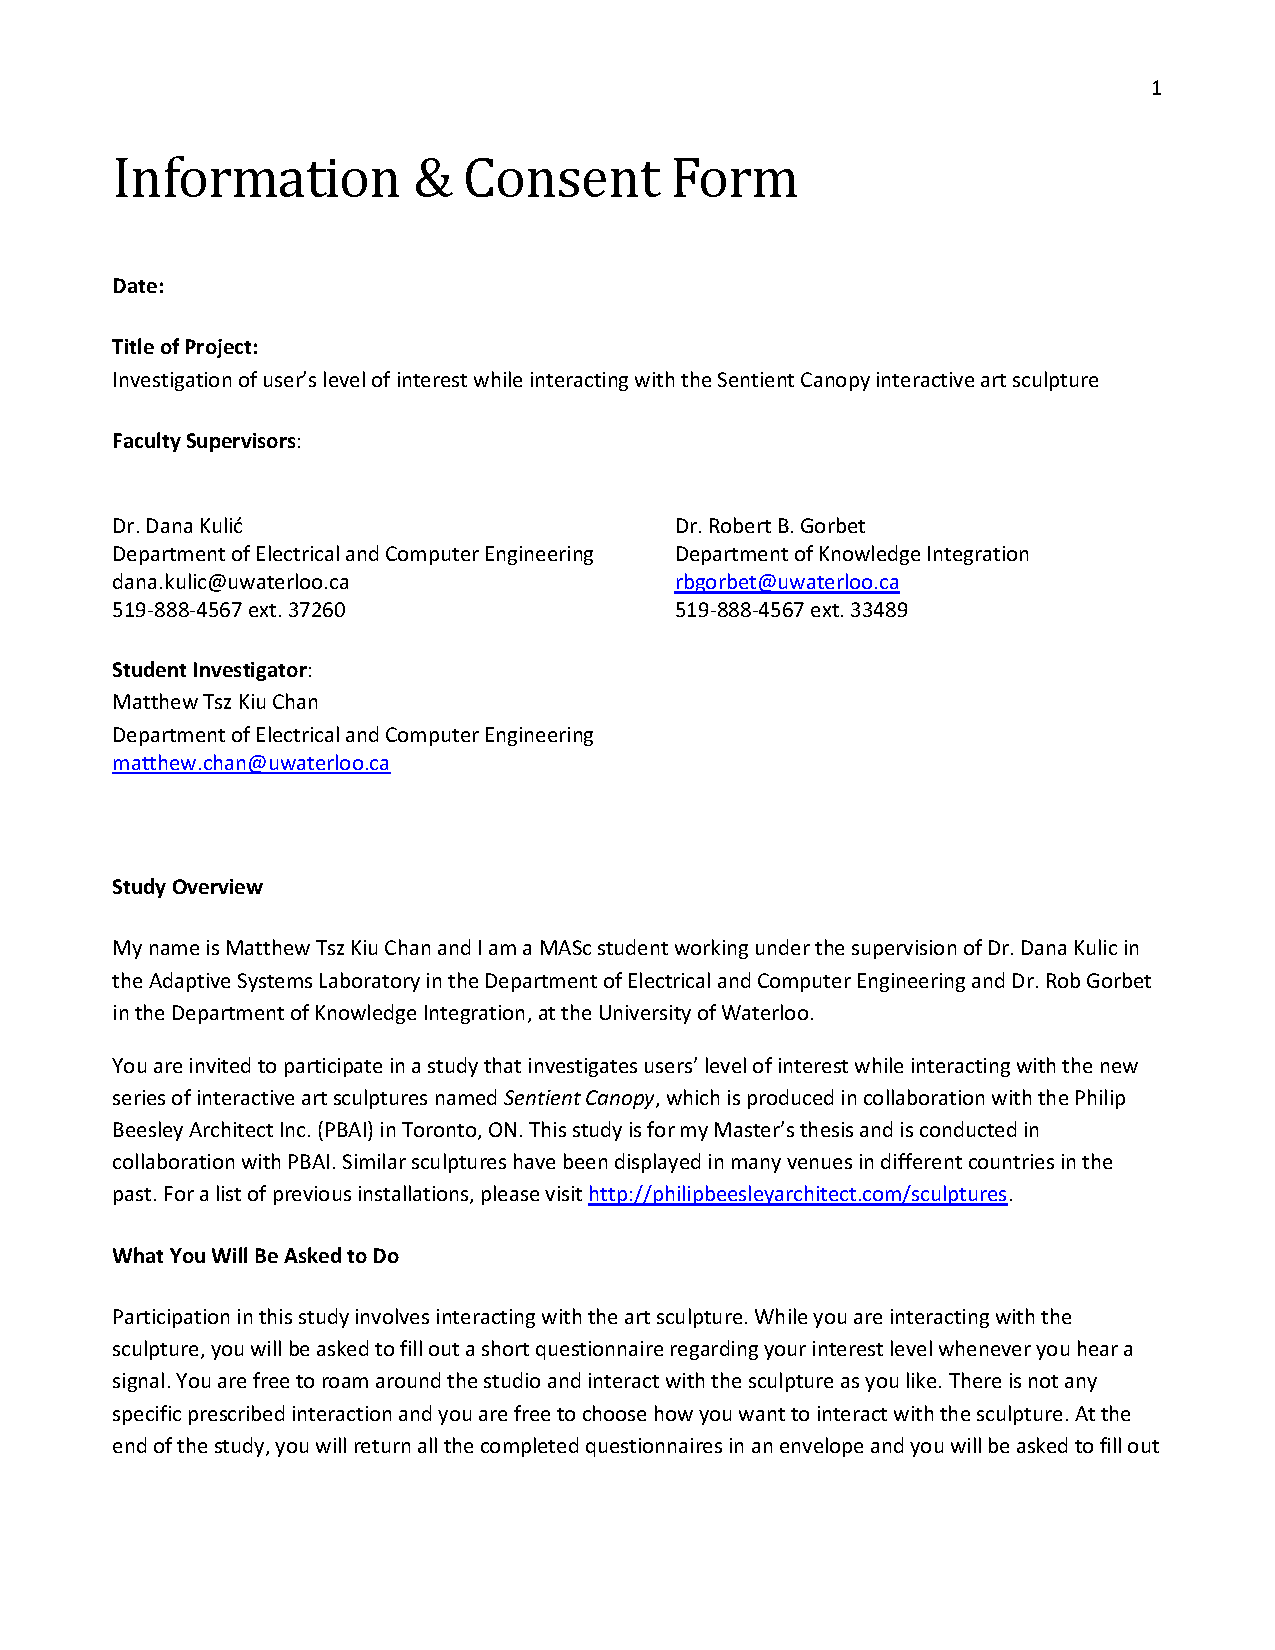
\includepdf[frame=true, scale=.75, pages={-}]{pdf/information_and_consent_form.pdf}
	\section{Exit Questionnaire}\label{Append:User Study Materials exit-survey}
	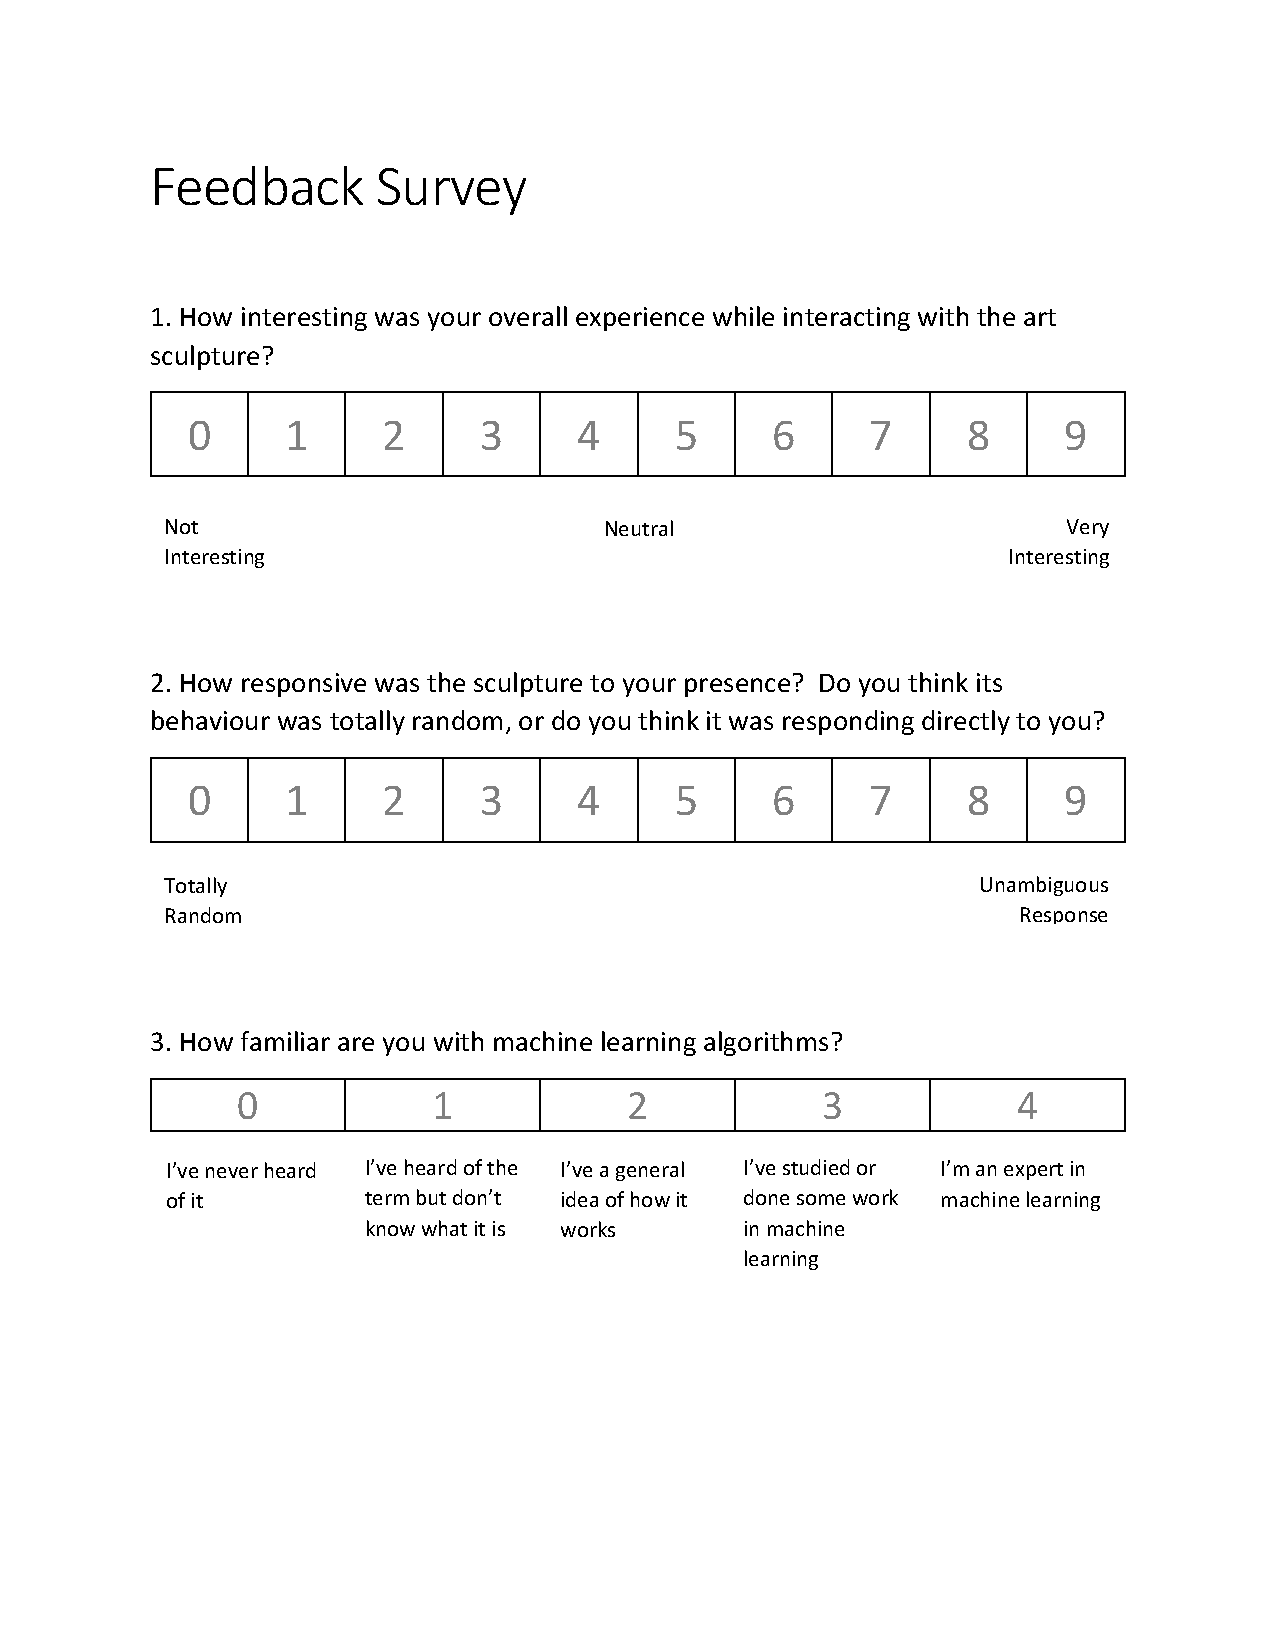
\includepdf[frame=true, scale=.75, pages={-}]{pdf/exiting_survey.pdf}
	\section{Debriefing Letter}\label{Append:User Study Materials debriefing}
	
\includepdf[frame=true, scale=.75, pages={-}]{pdf/debriefing_letter.pdf}
	
	\chapter[User Study Exit Questionnaires Written Responses]{User Study Exit Questionnaires Written Responses}\label{Append:User Study Written Responses}
	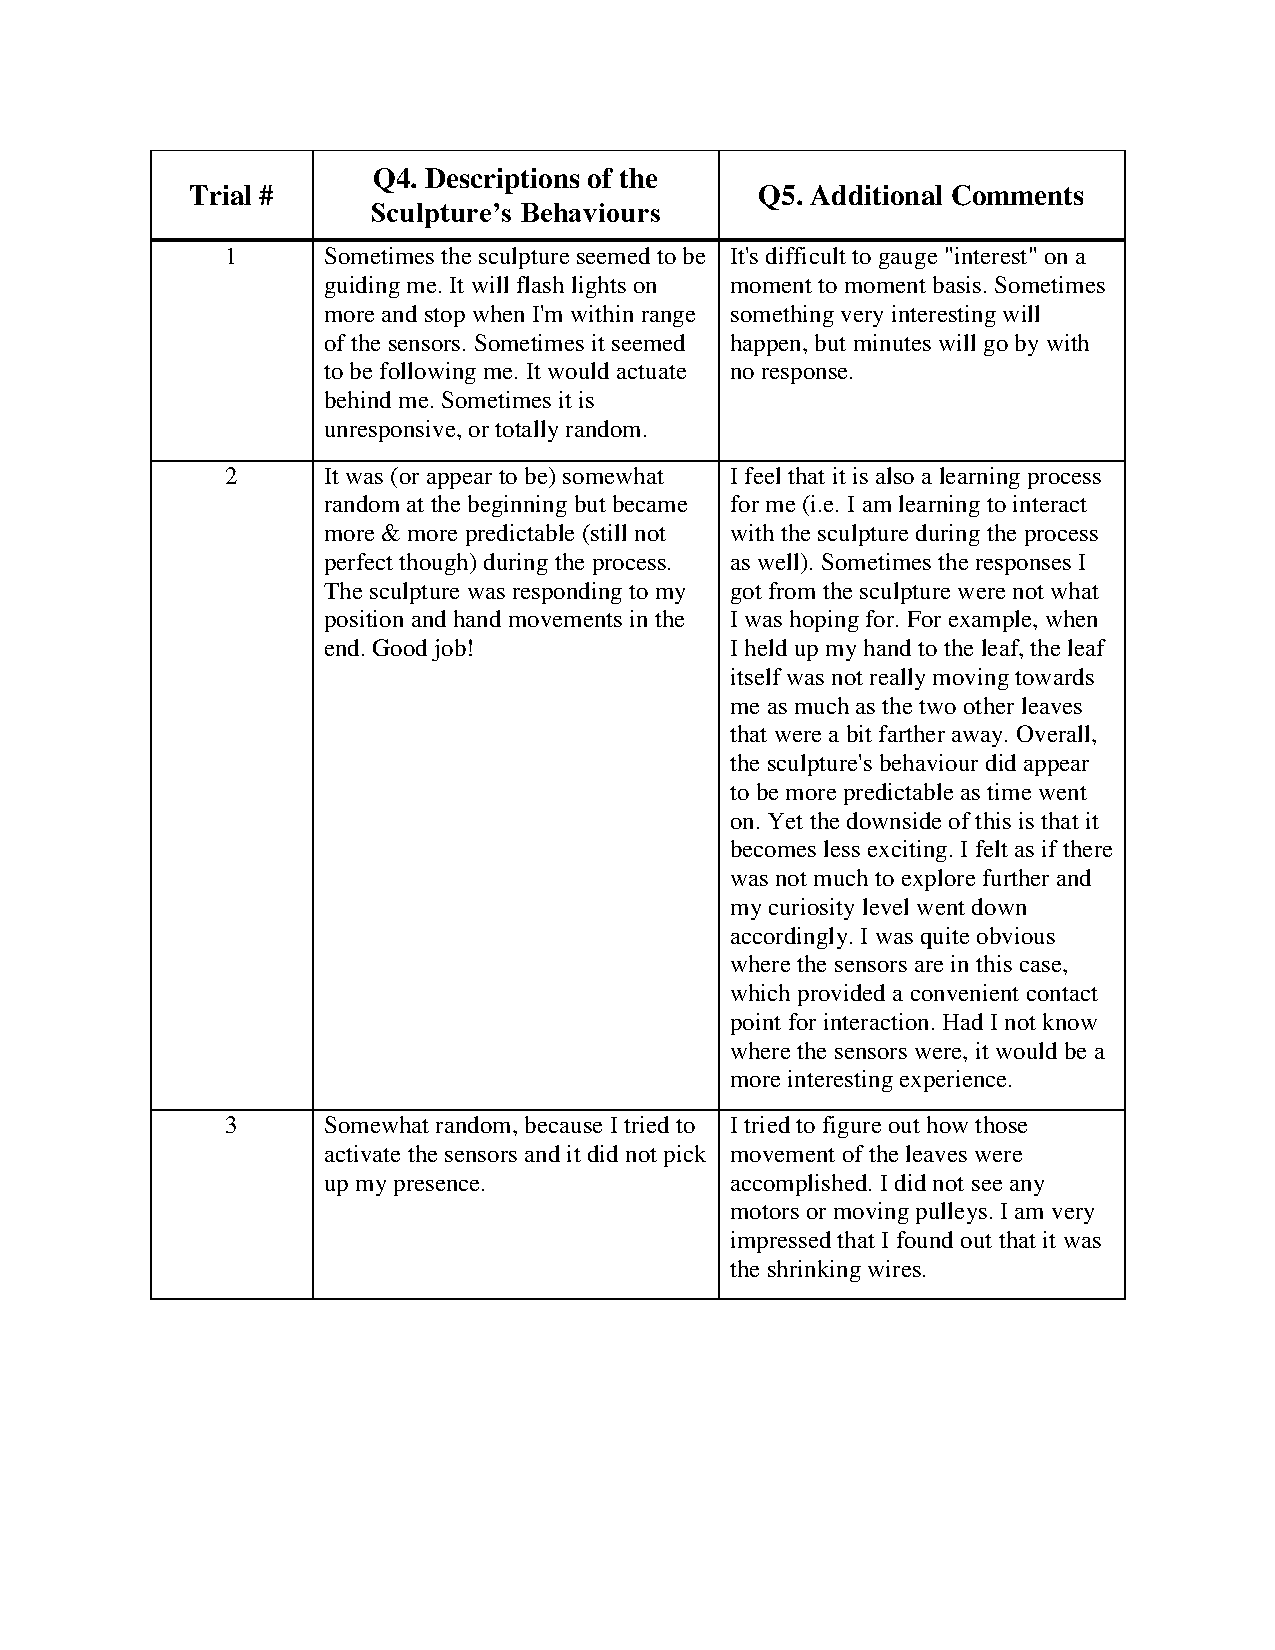
\includepdf[frame=false, scale=1.0, pages={-}, pagecommand={}]{pdf/exit_survey_responses.pdf}
	
	%----------------------------------------------------------------------
	% END MATERIAL
	%----------------------------------------------------------------------
	
	% B I B L I O G R A P H Y
	% -----------------------
	
	% The following statement selects the style to use for references.  It controls the sort order of the entries in the bibliography and also the formatting for the in-text labels.
	\bibliographystyle{IEEEtran}

	
	% This specifies the location of the file containing the bibliographic information.  
	% It assumes you're using BibTeX (if not, why not?).
	\cleardoublepage % This is needed if the book class is used, to place the anchor in the correct page,
	% because the bibliography will start on its own page.
	% Use \clearpage instead if the document class uses the "oneside" argument
	\phantomsection  % With hyperref package, enables hyperlinking from the table of contents to bibliography             
	% The following statement causes the title "References" to be used for the bibliography section:
	\renewcommand*{\bibname}{References}
	
	% Add the References to the Table of Contents
	\addcontentsline{toc}{chapter}{\textbf{References}}
	
	\bibliography{bib/Thesis}

	% Tip 5: You can create multiple .bib files to organize your references. 
	% Just list them all in the \bibliogaphy command, separated by commas (no spaces).
	
	% The following statement causes the specified references to be added to the bibliography% even if they were not 
	% cited in the text. The asterisk is a wildcard that causes all entries in the bibliographic database to be included (optional).
	%\nocite{*}
	
\end{document}
